\section{Visión}

\subsection{Introducción}
En esta sección exhibimos el sistema de analisis de imágenes por 
el cual el robot en cuestión da cuenta de la existencia o ausencia de 
elementos residuales en el entorno descripto. El sistema se basa en la 
utilización de una cámara de tipo webcam con una única lente para 
obtener información del ambiente. Esta información es luego procesada 
por una computadora a bordo del robot utilizando un algoritmo de visión 
cuyo único objetivo es la detección de residuos 
en las imágenes obtenidas. El sistema fue probado con la detección de 
colillas de cigarrillo, vasos descartables y platos de plástico. Para 
el desarrollo del algoritmo utilizamos la libreria de visión 
computacional OpenCV \cite{opencv_library} acompañado de un sistema 
desarrollado en C++. Como plataforma utilizamos un sistema linux 
ubuntu versión 9.10 corriendo en una netbook con procesador intel atom 
n450 y 1 gb de memoria RAM.
Esta sección se divide en las siguientes partes: en la sub-sección 2 se 
muestran los trabajos previos estudiados, en la sub-sección 3 se 
describe el algoritmo de detección, en las secciones 4 y 5 se explican 
los módulos de predicción y focalización mientras que en la 
sub-sección 6 se muestran los resultados. La sub-sección 7 concluye 
el cápitulo de visión.

\subsection{Trabajos previos}
En esta sección mostramos la información obtenida a partir de 
trábajos anteriores relacionados con visión computacional, 
procesamiento de imágenes y robots autonomos.
 
	%~ \subsubsection{A tale of two object recognition methods for mobile 
	%~ robots- Arnau Ramisa}
	%~ Este trabajo trata el problema de reconocimiento de objetos en un 
	%~ contexto hogareño. El autor introduce este problema argumentando 
	%~ que existe una gran cantidad de algoritmos para reconocimiento de 
	%~ objetos pero pocos de estos son apropiados para robots moviles. 
	%~ Entre estos se destacan el método de constelación utilizado con 
	%~ los detectores de puntos de interes de SIFT \cite{sift} y la bolsa 
	%~ de caracteristicas propuesto por Nister y Stewenius \cite[nister]. 
	%~ Con el objetivo de medir la performance de estos dos algoritmos, 
	%~ se recrea un ambiente hogareño compuesto por tres categorías de 
	%~ objetos: texturados, no texturados, y con texturas repetitivas. 
	%~ Cada objeto utilizado tiene 20 imágenes de entrenamiento y cada 
	%~ categoría contiene 3 objetos distintos. Luego se obtienen imágenes 
	%~ de prueba de estos objetos bajo condiciones de oclusión, cambios 
	%~ de iluminación, distintas perspectivas y otros tipicos ruidos 
	%~ encontrados por un robot movil atravesando un entorno. De cada una 
	%~ de estas imágenes se consideraron dos versiones, una versión con 
	%~ un recorte rectángular del objeto que incluye, inevitablemente, 
	%~ pixeles correspondientes al entorno de los objetos y una 
	%~ segmentación precisa utilizando los bordes de los objetos. Los 
	%~ resultados indican que utilizando el método de Lowe se obtienen 
	%~ mejores resultados con las imágenes rectángulares ya que se todas 
	%~ las ocurrencias de los objetos texturados fueron reconocidas y  
	%~ también algunos de los objetos con texturas repetitivas. Sin 
	%~ embargo, no se reconocieron objetos sin textura. Para el método de 
	%~ la bolsa de caracteristicas 
	\subsubsection{\label{volunteer}Mobile Field Robot with Vision-Based Detection of Volunteer Potato Plants in a Corn Crop - FRITS K. VAN EVERT}
	El objetivo de este trabajo es la construcción de un robot de 
	tamaño reducido y de bajo costo capaz de detectar un tipo de 
	planta de papas (volunteer potato) en un campo de trigo y propocionar control automático de esta planta. El interés en 
	esta especie se debe a que esta planta resulta dificil de controlar en las cosechas y favorece la 
	proliferación de otras sustancias que pueden perjudicar otros 
	cultivos. Con este proposito, se utilizó un camión de jugete como 
	soporte para un robot autónomo movil. Las partes de 
	radio-control del mismo fueron 
	removidas y remplazadas por micro-controladores para manejar la 
	dirección y la velocidad del robót. Además, como instrumento de 
	sensado se agregaron: una webcam estándar montada sobre un mástil a 
	una altura de 1.5m, un contador de revoluciones y un gyroscopio de 
	estado sólido. Las imágenes tomadas por la webcam son procesadas 
	por una pc a bordo con un procesador pentium M de 1.6 mhz. El control robotico de volunteer potatoes involucra al 
	menos 3 grandes etapas: navegación a travez del cultivo, detección 
	de plantas de papa y el control de las mismas.\\
	\indent En los campos de trigo la cosecha se dispone en filas 
	dejando espacio entre hilera e hilera para el paso del robot. Para 
	que este pueda navegar correctamente debe poder reconocer dichas 
	hileras de modo de orientarse correctamente en el cultivo. Esto se 
	logra mediante un algoritmo de visión. Este comienza 
	tomando una imágen RGB de 320x240 de la cámara. Para separar las 
	plantas del fondo se toma el doble del valor del canal G  y se 
	sustraen los canales rojos y azules (2G -R - B). Pixeles con un 
	valor mayor a cierto umbral son considerados planta y todos los 
	demás fondo. En un segúndo paso de procesamiento, se detectan las 
	filas de plantas utilizando un algoritmo inspirado en la 
	transformada de Hough \cite{hough62}. Este dibuja líneas imaginarias sobre la 
	imagen segmentada y se establece un puntaje para cada una según 
	cuantos pixeles blancos ( plantas) cubran. Estos puntajes se 
	convierten en valores de pixeles de una nueva imagen en donde la 
	coordenada vertical de cada pixel corresponde con la pendiente de 
	la línea imaginaria y donde la coordenada horizontal con la 
	intersección con el eje de coordenadas. Las hileras de plantas 
	contribuyen pixeles a varias líneas imaginarias y aparecen en la 
	nueva imagen como áreas con pixeles brillantes. Se utilizan las 
	operaciones de threshold y dilatación para combinar estas áreas 
	brillantes en un única región contigua de la cual se 
	extrae el centro de gravedad para representar una hilera de 
	plantas. Ya que el ruido puede ocasionar el reconocimiento de 
	hileras de plantas inexistentes se utilizan algunas reglas 
	sencillas para validar estas detecciones. Dos ejemplos de estas 
	reglas son ``las hileras de plantas deben estar a uno de los dos 
	costados del robot'' y ``las hileras deben ser paralelas entre si''.
	Luego, la orientación del robot se establece según la pendiente de 
	estas líneas.\\
	\indent Para la detección de las plantas ``volunteer potato'' se 
	utiliza una segunda cámara ubicada a una menor altura para obtener 
	mayor resolución sobre las plantas en si. El algoritmo consiste en 
	extraer las siguientes caracteristicas de las imágenes: (1) 
	promedio de rojo para pixeles de planta ,(2) promedio de verde para 
	pixeles de planta ,(3) promedio de azul para pixeles de planta, (4) 
	número total de pixeles de planta en la imagen binaria ,(5) número 
	total de pixeles de contorno en la imagen binaria y (6) número 
	total de pixeles de borde en la imagen Canny binaria. Estas 
	caracteristicas se relacionan al color(1,2 y 3), tamaño (4), figura 
	(combinación de 4 y 5) y textura (6).  Utilizando la misma fórmula 
	(2G -B -R) y la operación de threshold se segmenta nuevamente la imagen 
	 en pixeles de planta o fondo. Sobre esta imagen se calcula el 
	 promedio de rojo,azul y verde para las carateristicas 1,2 y 3. 
	 Contando el número de pixeles planta en la misma 
	 imagen se obtiene la caracteristica 4. Para la caracteristica 5 
	 se extraen los contornos de esta imagen y se cuenta el número de 
	 pixeles plantas contenidos en ellos. Finalmente, para la caracteristica 6 se 
	 repite este último procedimiento pero extrayendo los bordes de la 
	 imagen pero  
	 utilizando una implementación del algoritmo de Canny 
	 \cite{Canny:1986:ACA}. Se espera que el número de pixeles de 
	 borde sea mayor si se trata de una planta de papa ya que esta 
	 contiene un número mayor de hojas pequeñas que se solapan entre si 
	 mientras que las de trigo solo contienen algunas pocas hojas. Para 
	 clasificar las imágenes se uso un set de imágenes de entrenamiento
	 que fueron clasificadas manualmente según contenían 
	 plantas de papa o no. Luego se entrenó un 
	 clasificador de discriminante lineal de Fisher \cite{HastieEtAl2008} para distinguir 
	 entre imágenes que contienen plantas de papa de las que no.\\
	 \indent Para poner a prueba el algoritmo se tomaron dos sets de 
	 imágenes capturando el recorrido del mismo robot autónomo a 
	 travez de un campo de trigo. La tasa global de error para el 
	 clasificador fue de 1.5\% en el primer set y 10.6\% en el 
	 segúndo. En cuanto a la performance en la navegación, el robot 
	 fue capaz de recorrer con exito 120m de hileras de cultivo con 
	 una velocidad promedio de $0.67$ m/s. El autor remarca el alto 
	 tiempo de procesamiento requerido por el detector de plantas de 
	 papa ya que este bajó la tasa de cuadros del algoritmo de 
	 navegación de 30 a 8 cuadros/segúndo. Por dicho motivo se 
	 redujo la velocidad de desplazamiento del robot a 0.2 m/s para 
	 que este sea capaz de capturar correctamente todas las plantas. 
	 El mecanismo de control no fue implentado pero se incluyo un 
	 speaker que reproduce un sonido cuando este encuentra una planta 
	 del tipo buscado. Los algoritmos de visión utilizados fueron 
	 desarrollados usando Matlab con la librería Delft \cite{DipLib}.
	 
	\subsubsection{Review of shape representation and description techinques - Dengsheng Zhang}
El objetivo de este trabajo es realizar un resumen de las técnicas mas 
importantes en cuanto a la representación y descripción de figuras o 
formas.
Al clasificar dichas técnicas el autor sugiere una primera sub-división en 2 grupos, estos son: métodos basados en contornos y métodos basados 
en regiones. Los primeros se caracterizan por extraer  la información solo del contorno mientras que los segundos de la región completa abarcada
por el mismo. Dentro de cada clase, se dividen en técnicas 
estructurales o técnicas globales según  se represente una figura como un todo o 
por segmentos o secciones. La jerarquía completa puede observarse en la figura \ref{fig:review_shape}.\\
\indent Dentro de la categoría de los basados en contornos, en la sub-categoría de globales, los métodos suelen computar vectores de 
propiedades númericas extraidas de la información del borde de una 
figura. La comparación entre formas se realiza 
generalmente utilizando distancias métricas, como la distancia euclideana. Ejemplos de métodos sencillos que caen dentro de esta 
categoría son \textit{area, circularidad( $perimetro^2 / area$), 
excentricidad ( longitud del eje mayor / longitud del eje menor)}. Otros métodos 
de la misma familia pero mas complejos son los métodos basados en la correspondencia de puntos. En estos métodos se trata a cada punto como una 
caracteristica de la figura que compone. La distancia de \textit{ Hausdorff} es una técnica clasica de esta categoría. Dadas dos formas representadas
por dos sets de puntos $A={x_1,x_2...x_n}$ y $B={y_1,y_2...y_n}$ la distancia Haussdorf se define como 
\[
	 d_{\mathrm H}(A,B) = \max\{\,\sup_{x \in A} \inf_{y \in B} d(x,y),\, \sup_{y \in B} \inf_{x \in A} d(x,y)\,\}\mbox{,}
\] 

La comparación de figuras usando distancia Hausdorff resulta sensible 
al ruido y a pequeñas alteraciones en dos formas iguales. Existen otros métodos basados
en \textit{firma de contorno} que  representan una figura con una 
función uni-dimensional derivada de la información del borde de la 
misma, 
algunos son \textit{pérfil centroidal,coordenadas complejas y distancia al centroide}. Estos métodos deben ser normalizados para compensar
traslaciones o escalas lo que los hace relativamente costosos. Esto sumado a la sensibilidad al ruido y a pequeños cambios en los bordes, hace que el método 
no sea lo suficientemente robusto y que necesite de procesamiento adicional. Otra familia de descriptores se basan en los 
\textit{Momentos de borde}. Dada una parametrización como una función 
uni-dimensional $z(i)$, se define el momento \textit{r}-esimo \textit{$m_r$} 
y el momento central $\mu_r$ como:
\[
	m_r=\frac{1}{N} \sum_{i=1}^{N}{[z(i)]^r}\ \ \ \ \
	\mu_r=\frac{1}{N} \sum_{i=1}^{N}{[z(i) - m_1]^r}
\]

donde N es el número de puntos de borde. El momento normalizado $\bar{m_r}=m_r / (\mu_2)^{r/2}$
es invariante frente a traslaciones, rotaciones y escalamientos. Sin 
embargo, los momentos de alto orden
son dificiles de asociar con interpretaciones fisicas del contorno.\\
\indent La otra sub-categoría dentro de los métodos basados en contornos es la de los métodos estructurales.
En estos métodos se suele descomponer un contorno en segmentos de bordes llamado primitivas. Los métodos estructurales
entonces se diferencian entre si de acuerdo a la definicion y organización de estas primitivas. Algunos métodos
de descomposición son aproximación por polígonos, descomposición por curvatura, y ajuste de curva. El resultado
de la descomposición se codifica como una cadena $S=s_1,s_2...s_n$ donde $s_i$ puede ser un lado de un polígono, una 
arista cuadratica, una función spline, etc. Además, $s_i$ puede contener varios atributos como longitud,orientación, curvatura promedio,etc.
Métodos en esta línea son por ejemplo el de código en cadena, en el cual se describe un objeto por una serie de segmentos de longitud unitaria
con una orientación determinada. En su implementación, se superpone una imagen con una grilla y se aproximan los puntos del contorno al 
punto de la grilla mas cercano. Luego se selecciona un punto de 
partida y se codifica una secuencia estableciendo la dirección del segmento
que conecta un punto con el siguiente según la dirección de este en 
la grilla ( respecto del punto  anterior). Para la comparación de dos
contornos es necesario realizar normalizaciones ya que el punto de 
partida puede variar y frente a un cambio de escala pueden parecer 
contornos distintos. Otros métodos en esta sub-categoría pueden ser el de la descomposición polinomica o la descomposición en curvas suaves. \\
\indent Dentro de la categoría de los métodos basados en la región 
de una figura y la sub-categoría de globales podemos encontrar los \textit{momentos Hu}.
Un momento de Hu de un contorno 2d se define como:
\[
	m_{pq}=\sum_{x}{\sum_{y}{x^py^qf(x,y)}}
\]

Usando combinaciones lineales de momentos de Hu de ordenes bajos 
(valores de p y q menores a 2) se obtiene un descriptor 
invariante frente a rotaciones, traslaciones o escalamientos. Sin embargo esta técnica probó servir solo 
para figuras simples ya que en formas mas complejas no tiene una buena performance. Otros métodos en esta
sub-categoría pueden ser \textit{momentos algebraicos} o \textit{descriptor general de fourier}. En la otra sub-categoría de métodos
estructurales se destaca la \textit{envoltura convexa}. La envoltura convexa de un set de puntos es la mínima región que contiene 
dichos puntos y es convexa. Este método obtiene dicha región y la compara con el contorno original obteniendo una serie de pequeñas
componentes que marcan las deficiencias de concavidad del contorno. La 
figura en cuestión puede entonces representarse utilizando estas componentes.
Finalmente la comparación entre dos contornos representados con esta 
técnica resulta en la comparación de grafos lo cual es otro
problema a resolver por si solo. Además, métodos en esta familia son dificiles y complejos de implementar.\\
\indent Como conclusión el autor establece que los métodos basados en contorno son más populares ya que estan mas relacionados
a la percepción humana y que para muchas aplicaciones es solo necesario la información sobre el contorno y no sobre el interior del mismo.
Sin embargo, también establece que ya que solo usan parte de una figura, estos son más sensibles al ruido y pequeñas variaciones.

\begin{figure}[tpb]
\begin{center}
  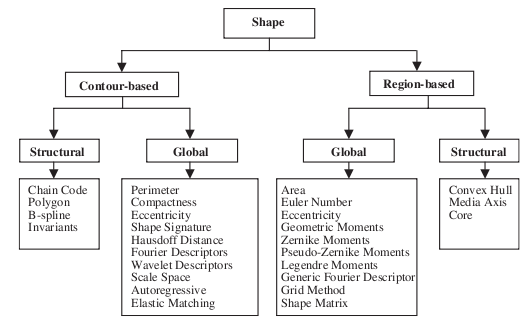
\includegraphics[scale=0.55]{figuras/shapess.png}
\end{center}
  \caption{Clasifación de las técnicas de descripción y representación de figuras}
  \label{fig:review_shape}
\end{figure}

% sidewalk following
	\subsubsection{\label{sec:sidewalk} Sidewalk Following Using Color Histograms - John S. Seng}
	Este trabajo describe un algoritmo  para detectar y seguir 
	veredas o áreas transitables en un video filmado, con el objetivo de 
	lograr la navegación autonoma de un robot dentro del 
	campus de una universidad. La plataforma en la cual se tomaron los videos esta 
	compuesta de una silla de ruedas motorizada controlada por una cpu 
	a bordo corriendo un sistema operativo linux. El robot tiene una 
	única cámara NTSC que provee imágenes color con una tasa de 15 
	cuadros por segundo. Todos los videos de prueba fueron tomados 
	utilizando esta plataforma conduciendola remotamente por un 
	operador a traves de un sistema de radio.\\
	\indent El algoritmo en cuestión utiliza histogramas 2-d de los 
	canales de tono y saturación de los pixeles para modelar las áreas
	transitables y las no transitables. Se utiliza un área de 
	entrenamiento ubicada directamente en frente del robot en la cual se asume que 
	no hay obstáculos y contiene pixeles representativos del área que 
	esta transitando. Esta área de entrenamiento se utiliza para 
	actualizar uno de los 4 histogramas que modelan el área 
	transitable. Además, se mantiene un histograma que modela el
	área no transitable o fondo de la imagen, tomando una muestra de pixeles del último 
	cuadro que fueron clasificados como tales . La 
	clasificación de pixeles entonces se realiza utilizando la 
	siguiente métrica:
	\[
	P_{transitable}= T(h,s)/ ( T(h,s) + NT(h,s))
	\]
	donde T y NT son los histogramas que modelan las áreas transitables
	y no transitables respectivamente. $P_{transitable}$ se calcula para 
	los 4 histogramas tomando el máximo de estos, si este supera 
	cierto umbral entonces se considera a dicho pixel como 
	correspondiente a un área transitable.
	La actualización de los histogramas se realiza reemplazando el 
	histograma de menor cantidad de aciertos con el histograma 
	del área de entrenamiento.  Entre los resultados se destaca el 
	hecho de que 4 histogramas resultaron suficientes para modelar la
	variación de color de las áreas transitables pero, sin embargo, este no 
	logro clasificar a la zonas cubiertas de sombra como transitables.
	Bajo condiciones de luz favorables, 2 histogramas fueron 
	suficientes para clasificar , en promedio, el 50\% del área 
	transitable. Las posibles mejoras incluyen la incorporación de 
	bordes o texturas para el reconocimiento de áreas transitables 
	como así la posibilidad de tener áreas de entrenamiento con 
	posiciones dinámicas de acuerdo a las condiciones de iluminación.
	
	
	
	
	\subsubsection{Skin Detection using HSV color space - V. A. Oliveira, A. Conci}
	En este artículo se trabajó sobre la detección de piel en imágenes utilizando el espacio de color HSV. El algoritmo propuesto 
por el autor consiste en el filtrado de los pixeles en base al valor del canal de tonalidad (canal H). Los rangos de valores utilizados para 
representar el color de la piel fueron obtenidos de otros artículos 
relacionados. Con el objetivo de eliminar ruido, se aplican filtros morfológicos y de suavizado, estos son (en este orden) dilatación, erosión y un filtro de mediana. Para los filtros morfológicos se utilizaron núcleos de 5x5 pixeles mientras que para el filtro de mediana se usaron núcleos de 3x3 pixeles. Finalmente, el autor midió la performance de su algoritmo utilizando imágenes de prueba en donde se aprecian distintas zonas con piel aisladas. A partir de estas imágenes, se obtuvieron las coordenadas de los pixeles que se corresponden con piel y se las contrastó con aquellas que identificó el algoritmo. Los resultados presentados para 4 imágenes son satisfactorios obteniendo en promedio un porcentaje de falsos negativos cercano al 1\% y de falsos positivos menor al 6\%.

	\subsubsection{Line Detection and Lane Following for an Autonomous Mobile Robot - Andrew Reed Bacha}
	En este artículo se describió el software utilizado para uno de los robots ganadores de la competencia "Intelligent Ground Vehicle Competition" (IGVC) en donde se requiere que los robots naveguen  a través de un camino delimitado por líneas pintadas sobre césped en un ambiente al aire libre en donde se pueden presentar obstáculos. El robot utilizaba una única cámara para el sistema de visión y su objetivo era detectar las líneas pintadas 
para determinar la dirección de movimiento del robot. El algoritmo 
descripto por el autor cuenta con una etapa de pre-procesamiento y otra 
de detección de líneas. En la etapa de pre-procesamiento se comienza 
por convertir la imagen a escala de grises utilizando una 
transformación en la que la intensidad de cada pixel es determinada 
usando $2*B(i,j) - G(i,j)$ con el argumento que el canal verde contiene 
ruido provocado por la exposición de luz en el pasto y de esta manera 
se lo elimina. Luego el autor propone utilizar un ajuste de brillo 
argumentando que los pixeles de la zona más alta se encuentran más 
expuestos a la luz por la perspectiva de la cámara, para esto sustrae 
una máscara que compensa este efecto. Además, el autor elimina la 
proyección del robot mismo sobre la imagen capturada por la cámara. 
En la etapa de detección se realizó un threshold para obtener los 
pixeles más brillantes. Luego, la salida del threshold se utilizó 
como entrada para un detector de líneas basado en el algoritmo de 
Hough \cite{hough62}. Finalmente, según la orientación de las líneas detectadas se determina la dirección del robot. El algoritmo se consideró exitoso ya que el robot propuesto fue el ganador de la competencia.
\pagebreak

	
\subsection{Algoritmo de detección}
En esta sección describimos las distintas etapas del algoritmo de análisis 
de imágenes utilizado. Estas se pueden separar en una etapa de 
pre-procesamiento donde se realiza un tratado de la imagen obtenida 
para re1saltar las caracteristicas de interes y  una segunda etapa donde se 
extraen estas caracteristicas para interpretarlas y  buscar 
los objetos residuales en las imágenes.

\subsubsection{Estructura general}
La figura \ref{fig:alg_steps} ilustra las etapas del algoritmo. Este fue programado utilizando el lenguaje C++ y la librería de visión computacional openCv.
El algoritmo comienza por tomar una imagen fresca de la cámara, las 
imágenes capturadas poseen el formato 24-bit RGB. Con el objetivo de 
minimizar el impacto producido por cambios en la iluminación se 
convierte la imagen al formato HSV (tono, saturación y brillo). Luego 
utilizamos el canal del tono de esta nueva imagen para establecer que 
pixeles se corresponden con el color buscado, filtrando aquellos 
pixeles que no coinciden con el rango deseado (ver inciso 
\ref{sec:color}). A su vez, usamos la información brindada por los  canales de saturación y/o brillo para obtener más precisión sobre el color de los pixeles.\\
	\indent Descartamos los pixeles filtrados en el canal de saturación 
	realizando un and bit a bit con la imagen filtrada.  En la siguiente 
	etapa, se utilizan filtros morfológicos cuyo objetivo es la 
	eliminación de ruido. El resultado de aplicar estos filtros resulta 
	en la expansión de las áreas donde hay mucha presencia de pixeles de 
	interés, produciendo un área de intensidad homogénea mientras que 
	en las áreas con poca presencia de estos 
	elimina la aparición aislada de los mismos, generados por el ruido (ver 
	inciso \ref{sec:morph}). El paso 
	siguiente consiste en la aplicación de un umbral. El umbral filtra 
	aquellos pixeles que no se encuentren por encima de un valor mínimo 
	de intensidad marcándolos con valor cero y conserva únicamente los 
	pixeles que si lo hacen estableciéndoles un valor predeterminado 
	(mayor a cero) (ver inciso \ref{sec:thresh}). \\
	\indent Las operaciones que mencionamos hasta aqui componen la 
	etapa de  pre-procesamiento de la imagen. Finalizada dicha etapa del 
	algoritmo deseamos tener solo pixeles de los potenciales objetos de 
	interés. Vale notar que, como consecuencia de aplicar un filtro 
	umbral, la imagen se encuentra binarizada, es decir, los pixeles solo 
	pueden tener dos posibles valores: cero (negro) si no es un pixel de 
	interés o mayor a cero en el caso contrario. Es entonces que 
	automáticamente quedan delimitadas las áreas que contienen pixeles 
	de interés, el próximo paso del algoritmo se encarga de obtener los 
	contornos de estas áreas. Para esto utilizamos el algoritmo de Suzuki 
	\cite{suzuki85} que recorre los bordes de estas zonas y crea 
	secuencias de puntos $(x,y)$ que definen el contorno de las mismas. 
	Las secuencias de puntos son luego aproximadas para generar polígonos 
	cerrados mediante el algoritmo de Douglas-Pecker \cite{dp74}. Tomando 
	estos polígonos definimos distintos parámetros tales como el área, 
	perímetro o figura que nos permiten discernir si se trata de un objeto 
	a reconocer o no. La posición del objeto es luego informada a 
	partir de su rectángulo contenedor mínimo.


\begin{figure}[tpb]
\begin{center}
  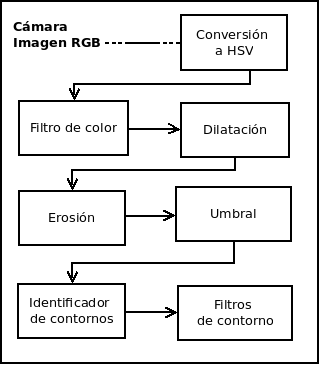
\includegraphics[scale=0.6]{figuras/vision-flow.png}
\end{center}
  \caption{Etapas del algoritmo de visión}
  \label{fig:alg_steps}
\end{figure}


\subsubsection{\label{sec:color} Detección de color}
El problema de decidir si un pixel determinado se corresponde con un 
color particular resulta mucho más sencillo de resolver en el espacio 
de color HSV. Este espacio de color se compone de un canal H que 
describe el color de un pixel, un canal S que pondera la saturación de 
dicho color y un canal V que mide la luminosidad de dicho pixel. En el espacio RGB, de haber un cambio en el brillo o 
iluminación de la imagen, los tres canales se ven afectados de igual 
manera mientras que en el espacio HSV el canal H, que codifica la 
información sobre el tono del color, se ve mucho menos influenciado en 
comparación con los otros dos canales ( saturación y valor). De esta 
manera, podemos caracterizar el color de un pixel determinado 
observando su valor en dicho canal sin molestarnos demasiado por las condiciones de brillo o iluminación al cual se encuentra expuesto.
\\ \indent Realizamos la detección de color verificando los valores correspondientes al canal H (tono) de la representación HSV de la imagen. Para esto realizamos la conversión de la imagen obtenida por la cámara  de formato RGB a HSV usando el algoritmo expuesto en la figura \ref{code:hsv}.
\begin{figure}[tpb]
\begin{verbatim}
V=max(R, G, B)
S=(V-min(R,G,B))*255/V   if V!=0, 0 otherwise

       (G - B)*60/S,  if V=R
H= 180+(B - R)*60/S,  if V=G
   240+(R - G)*60/S,  if V=B

if H<0 then H=H+360
\end{verbatim}
\caption{\label{code:hsv}pseudo-código de la conversión RGB-HSV}
\end{figure}

Obteniendo el canal H, nos fijamos que los valores de los pixeles 
estén dentro de cierto rango correspondiente al color que buscamos. 
Como podemos observar en la figura \ref{fig:hsv_space}, en el espacio 
de color HSV los colores se encuentran dispuestos a lo largo de una 
circunferencia, donde cada tonalidad representa un ángulo en la misma. 
Por ejemplo, si queremos abarcar las distintas tonalidades del azul 
podemos elegir el rango que va de 200$^\circ$ a 260$^\circ$. Cuando 
buscamos un color en particular  es preciso elegir este rango 
cuidadosamente ya que de ser un rango muy restrictivo podemos 
despreciar pixeles de interés arruinando la figura del contorno del 
objeto a buscar y si elegimos un rango más abarcativo podemos tomar 
pixeles de colores distintos al buscado, introduciendo ruido. 
Experimentalmente comprobamos los resultados de un filtro de color con 
distintos rangos, como se muestra  en la figura \ref{fig:hue_range}. 
Una vez obtenidos los pixeles que se corresponden con el color buscado 
se combinan estos con los del canal de saturación utilizando un and 
bit a bit entre ambos pixeles. A mayor saturación consideramos mayor 
presencia del color buscado en dicho pixel y por lo tanto mayor 
probabilidad de que este corresponda a el objeto buscado. \\
\indent En el caso de las colillas se utilizó el rango para el canal de tono 
$20<h<40$ con valor en el canal de saturación mayor a 60. En el caso 
de los platos y los vasos se busco detectar el color blanco. La 
particularidad de este color es que este se encuentra presente en 
todos los colores del rango H y se lo caracteriza por su valor alto en 
el canal de valor. Por este motivo, para platos y vasos solo se verifica que 
se cumpla que el valor del pixel tenga $v>170$.
\begin{figure}[tpb]
\begin{center}
  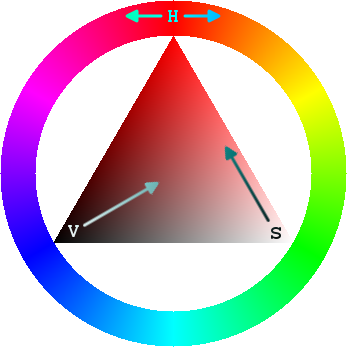
\includegraphics[scale=0.4]{figuras/hsv_triangle.png}
\end{center}
  \caption{\small Espacio de color HSV. Los distintos tonos de colores se encuentran dispuestos a lo largo de la circunferencia.}
  \label{fig:hsv_space}
\end{figure}

\begin{figure}[tpb]
\begin{center}
  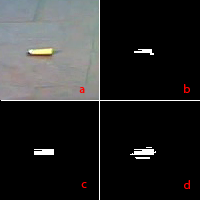
\includegraphics[scale=0.8]{figuras/hue.png}
\end{center}
  \caption{\small Resultados de aplicar un filtro de color utilizando distintos rangos. (a) Captura original. (b) Resultado de aplicar el filtro $35\le h \le45$, se pierden algunos pixeles. (c) Resultado de aplicar el filtro $20\le h \le40$. (d) Resultado de aplicar el filtro $10 \le h \le 50$, se introducen pixeles extra.} 
  \label{fig:hue_range}
\end{figure}

	\subsubsection{\label{sec:thresh} Threshold}
Threshold o umbral es una operación que nos permite pasar de una 
imagen en escala de grises a una imagen binaria. El proceso de 
thresholding consiste en distinguir los pixeles que se encuentran por 
encima de un cierto valor de los que están por debajo del mismo. Con este objetivo, se crea una imagen binaria asignándoles valores 1 o 0 según su condición respecto del valor. El algoritmo de thresholding nos puede servir para distinguir un objeto determinado de un contexto o fondo siempre y cuando el objeto posea un mayor brillo que el fondo en el que se encuentra. Esto significa que los pixeles correspondientes a un objeto se encontrarán por encima de cierto valor característico, determinado por el fondo. En nuestro caso esto no sucede de esta forma ya que no siempre la intensidad o brillo de los objetos supera al fondo en el que se encuentra, por lo cual resulta difícil utilizar esta técnica. Podemos apreciar un ejemplo de este efecto en la figura \ref{fig:thresh-dif}. \\
\indent Existen diversas variantes de threshold, los parámetros 
utilizados son $V$ para indicar el valor umbral y $M$ que indica el 
valor a tomar por los pixeles.
\begin{itemize}
\item{ Threshold binario:  Si un pixel se encuentra por encima de $V$, se le asigna un valor $M$, de otro modo se le asigna $0$.}
\item{ Threshold binario invertido:  Si un pixel se encuentra por encima de $V$, se le asigna 0, de otro modo se le asigna $M$.}
\item{ Threshold truncado:  Si un pixel se encuentra por encima de $V$, se le asigna $V$, de otro modo conserva su valor.}
\item{ Threshold a cero invertido : Si un pixel se encuentra por encima de $V$ se le asigna $0$, de otro modo, conserva su valor.}
\item{ Threshold a cero invertido : Si un pixel se encuentra por encima de $V$ conserva su valor, de otro modo se lee asigna $0$.}
\end{itemize}
El problema con esta familia de algoritmos es que en todos los casos el 
valor $V$ permanece constante para toda la imagen haciéndolo propenso 
a errores cuando la imagen presenta diferentes niveles de iluminación. 
Una manera de solucionar esto es pre-computando el valor $V$ para 
distintas zonas de la imagen como lo hace la 
técnica de thresholding adaptativo, que computa el valor de $V$ a 
medida que recorre la imagen, usando para esto, una ventana cuyo 
tamaño es definido por el usuario. Siguiendo esta lógica, se utilizan 
los valores de los pixeles abarcado por esta ventana para definir un valor 
de $V$ (por ejemplo calculando el promedio de intensidad) y luego se 
aplica alguna de las técnicas de thresholding simples mencionadas, 
utilizando este mismo valor. Sin embargo, este algoritmo es más 
costoso y puede provocar efectos indeseados como se observa en la 
figura \ref{fig:thresh_adapt} en donde el valor de V se calcula 
utilizando un promedio ponderado por una función gaussiana de acuerdo a la distancia del centro 
de la ventana.\\
\indent En nuestro caso, utilizamos thresholding no para distinguir los 
objetos del fondo (esto es trabajo del filtro de color), sino como 
método de eliminación de ruido. Cuando se combina el canal de 
saturación con el resultado del filtro de color, se obtiene una imagen 
de escala de grises que esta segmentada en un conjunto de áreas con 
distintos valores de intensidad. Luego de aplicar dilatación y 
erosión, los niveles de intensidad de cada área se vuelven 
homogéneos (ya que se toma el máximo o mínimo local) y es entonces 
donde podemos diferenciar las zonas de intensidad alta de las zonas de 
intensidad baja, motivo por el cual utilizamos la operación de 
threshold. En las figuras \ref{fig:threshold_ruido} y 
\ref{fig:threshold} exhibimos dos casos de utilización de threshold. 
Para la detección de colillas, vasos y platos utilizamos establecemos 
el umbral de la operación de threshold en 100, asignandoles un valor 
de 255 (valor máximo) a los pixeles que superen dicho umbral o 0 en 
caso en contrario. 
\begin{figure}[tpb]
\begin{center}
  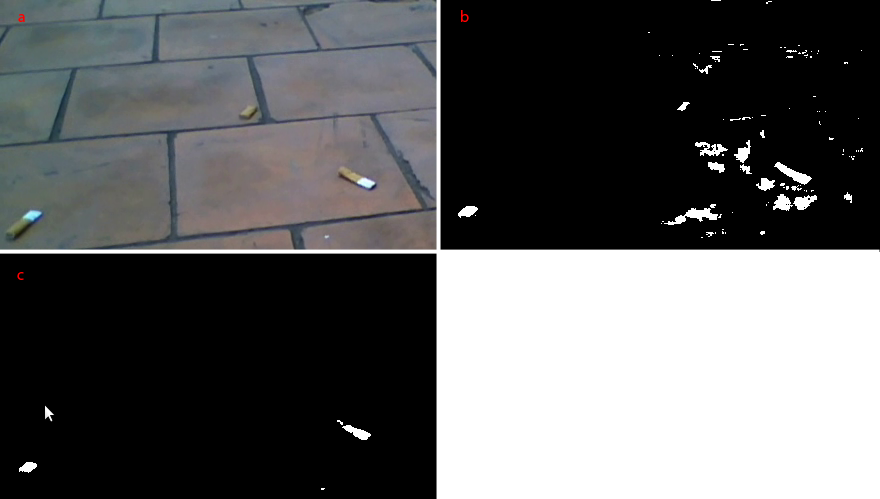
\includegraphics[scale=0.4]{figuras/threshold-dif.png}
\end{center}
  \caption{\small Distintos valores de umbral. (a) Captura original. 
  (b) Threshold binario con umbral 120. Se observan pixeles extra en 
  la detección. (c) Threshold binario con umbral 160. Se observa la 
  ausencia de pixeles. }
  \label{fig:thresh-dif}
\end{figure}

\begin{figure}[tpb]
\begin{center}
  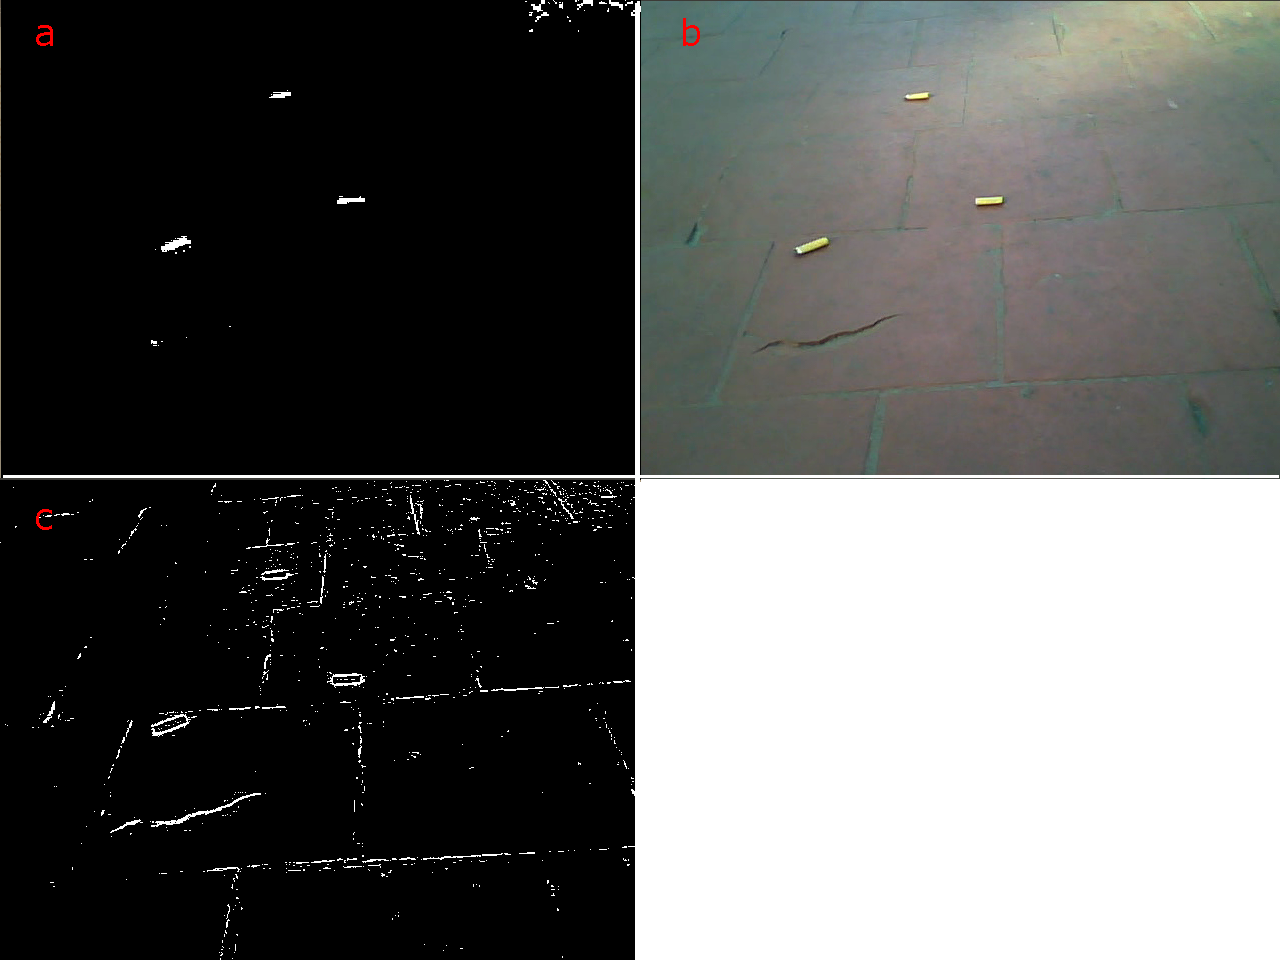
\includegraphics[scale=0.25]{figuras/adaptative.png}
\end{center}
  \caption{\small Comparación de threshold adaptativo con el filtro de 
  color. (b) Imagen obtenida de la cámara. 
  (a) Salida del filtro de color. (c) Threshold adaptativo sobre la 
  imagen b previa conversión a blanco y negro utilizando una ventana 
  de 9x9 pixeles. Se observa que el filtro adaptativo identifica 
  correctamente los contornos de las colillas pero agrega mucha 
  información redundante que resultara en procesamiento extra.}
  \label{fig:thresh_adapt}
\end{figure}


\begin{figure}[tpb]
\begin{center}
  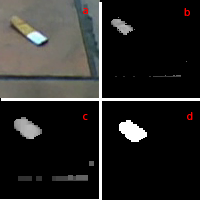
\includegraphics[scale=0.8]{figuras/threshold-ruido.png}
\end{center}
 \caption{\small Resultados de aplicar thresholding binario. (a) Captura original. (b) Salida del detector de color, se observan algunos pixeles extra cerca de la línea de brea. (c) Salida de la operación de dilatación-erosión. (d) Salida de la operación de thresholding binario con un umbral de $100$. La baja intensidad de los pixeles extra en la línea de brea no supera el umbral propuesto y por lo tanto son descartados. El contorno del objeto de interés se conserva aislado.} 
  \label{fig:threshold_ruido}
\end{figure}

\begin{figure}[tpb]
\begin{center}
  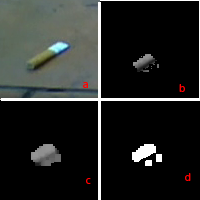
\includegraphics[scale=0.8]{figuras/threshold.png}
\end{center}
  \caption{\small Resultados de aplicar thresholding. (a) Captura original. (b) Salida del detector de color, se observan algunos pixeles extra debajo del objeto de interés. (c) Salida de la operación de dilatación-erosión, los pixeles extra se combinaron con los pixeles del objeto.(d) Salida de la operación de thresholding binario con un umbral de $100$. La baja intensidad de los pixeles extra en la zona debajo del objeto no supera el umbral propuesto y por lo tanto son descartados. El contorno del objeto de interés se conserva aislado.} 
  \label{fig:threshold}
\end{figure}

	\subsubsection{\label{sec:morph} Operaciones morfológicas}
Sombras, luces y otros efectos pueden alterar el resultado del filtro de color introduciendo ruido en los objetos a detectar. Este ruido puede surgir tanto de la omisión de pixeles de interés como por la inclusión de pixeles extra. Para subsanar esto, utilizamos las operaciones morfológicas de dilatación y erosión. Ambas se basan en la utilización de un elemento estructural, esto es, una figura de cualquier tamaño y forma que tiene definido un punto principal y que recorre la imagen solapándose pixel a pixel. De acuerdo a operaciones locales a este elemento, el pixel que coincide con el punto principal se ve modificado. Usualmente se utilizan como elementos estructurales, pequeños discos o cuadrados, donde el punto principal se encuentra en el centro del mismo. El efecto generado se entiende mejor observándolo en imágenes binarias. En el caso de la dilatación, la idea intuitiva es remplazar cada pixel no vacío con una copia del elemento estructural cuyo punto principal se encuentra en esa posición. Para la erosión, la idea intuitiva es quedarse con aquellos pixeles tal que podamos hacer caber un elemento estructural cuyo punto principal se encuentra en esa posición y dicho elemento solo cubra pixeles no vacíos.
Ilustramos esto en las figuras \ref{fig:dilate-sample} y \ref{fig:erode-sample}.


\begin{figure}[tpb]
\begin{center}
  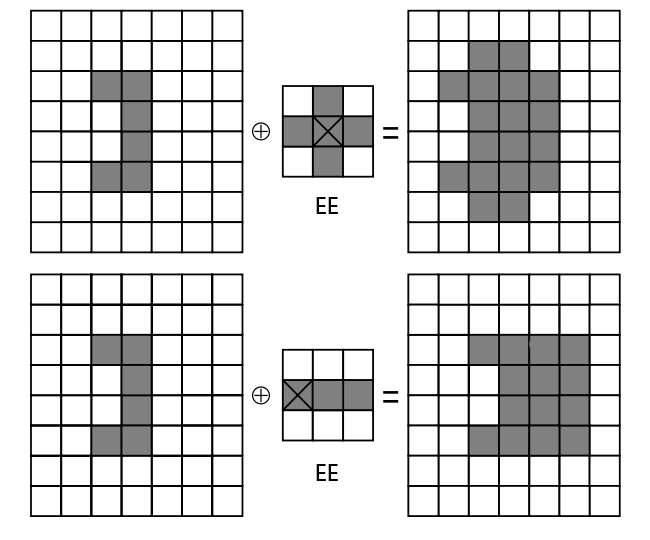
\includegraphics[scale=0.4]{figuras/dilate-sample.png}
\end{center}
  \caption{\small Operación de dilatación en imágenes binarias. Se reemplazan los pixeles no vacíos por una copia del elemento estructural con punto principal en esa posición. La cruz indica la posición del punto principal dentro del elemento estructural (ee). Imagen obtenida del curso de visión artificial de la Universidad Politécnica de Madrid.}
  \label{fig:dilate-sample}
\end{figure}

\begin{figure}[tpb]
\begin{center}
  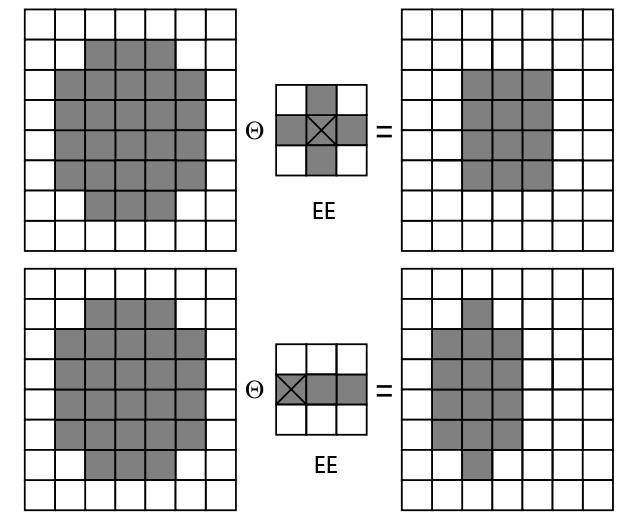
\includegraphics[scale=0.4]{figuras/erode-sample.png}
\end{center}Podemos apreciar un ejemplo de threshold en la figura \ref{fig:threshold}
  \caption{\small Operación de erosión en imágenes binarias. Se persisten los pixeles no vacíos en donde cabe una copia del elemento estructural cuyo punto principal se encuentra en esa posición. La cruz indica la posición del punto principal dentro del elemento estructural (ee). Imagen obtenida del curso de visión artificial de la Universidad Politécnica de Madrid. } 
  \label{fig:erode-sample}
\end{figure}

	\paragraph{Dilatación}
En imágenes no binarias, la operación de dilatación se define 
tomando el máximo local bajo el elemento estructural y asignandole ese valor al punto principal. El efecto producido es una reducción general en el brillo de la imagen y un probable aumento el tamaño de las figuras \cite{nasa-dilate-erode}.  Cuando un área grande aparece, a causa del ruido, partida en varias componentes, el uso de la operación de dilatación provoca que  se combinen nuevamente en una sola. Un ejemplo de esto puede ser apreciado en la figura \ref{fig:dilate}. Otro beneficio de utilizar dilatación es la eliminación del ruido espurio como se aprecia en la figura \ref{fig:dilate-ruido}.

\begin{figure}[tpb]
\begin{center}
  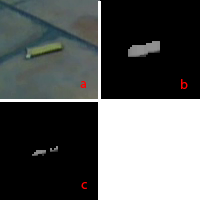
\includegraphics[scale=0.8]{figuras/dilate1.png}
\end{center}
  \caption{\small Efecto de la operación de dilatación. (a)  Imagen original tomada de la cámara. (b) Imagen luego de aplicar dilatación a la imagen c con un elemento estructural cuadrado de 3x3 pixeles, con punto principal en el centro. (c) Salida del filtro de color. La colilla de cigarrillo esta 'partida' en dos componentes conexas. } 
  \label{fig:dilate}
\end{figure}

\begin{figure}[tpb]
\begin{center}

  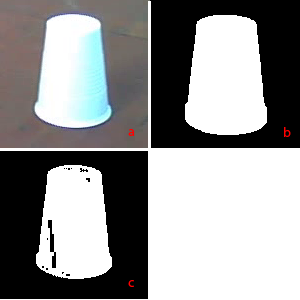
\includegraphics[scale=0.6]{figuras/dilate-ruido.png}
\end{center}
  \caption{\small Eliminación de ruido mediante la operación de dilatación. (a) Imagen original tomada de la cámara. (b) Imagen luego de aplicar dilatación a la imagen c con un elemento estructural cuadrado de 3x3 pixeles, con punto principal en el centro. (c) Salida del filtro de color. Observamos áreas  oscuras en el interior del vaso. }
  \label{fig:dilate-ruido}
\end{figure}

	\paragraph{Erosi\'on}
En imágenes no binarias, la operación de erosión se define tomando el mínimo local bajo el elemento estructural y poniéndole ese valor al punto principal. Contrario a la dilatación, este operador generalmente reduce el brillo de la imagen y disminuye el tamaño de las figuras \cite{nasa-dilate-erode}. Usamos la operación de erosión para eliminar las protuberancias que pueden surgir de aplicar la operación de dilatación. En la figura \ref{fig:erode} podemos apreciar el efecto de aplicar dilatación y luego erosión.

\begin{figure}[tpb]
\begin{center}
  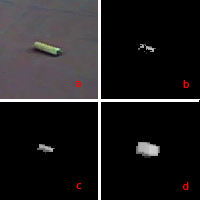
\includegraphics[scale=0.8]{figuras/erosion.png}
\end{center}
  \caption{\small Ejemplo de erosión. (a) Captura original. (b) Salida del filtro de color. Se observan fallas en la detección del objeto. (d) Se aplica la operación de dilatación a la imagen b. Se observa la producción de protuberancias en la figura del objeto. (c) Salida luego de aplicar erosión a c. La figura del objeto se corrige eliminando parte de las protuberancias. Sin embargo, no se observan fallas en la detección del objeto. }
  \label{fig:erode}
\end{figure}

	\subsubsection{Detección de contornos}
	La detección de contornos se realiza sobre las imagenes binarias producidas en la etapa de pre-procesamiento. Dichos contornos
	quedan definidos implicitamente como la separación de regiones 
	positivas de las negativas \footnote{ Como se trata de imágenes 
	binarias, llamamos a una región positiva a las que contienen 
	pixeles con valores mayores a 0 y a las negativas a las que tienen 
	un valor de 0.}. Por lo tanto para obtener estas secciones hacemos 
	uso de los algoritmos explicados en esta sub-sección.
	
	\paragraph{Algoritmo} 
	Recordemos que las imágenes binarias se caracterizan por tener solo 
	dos tipo de pixeles, los que tienen un valor de 0 o los que tienen 
	un valor mayor a 0. Denominamos a estos pixeles como 
	0-pixeles o 1-pixeles respectivamente. Decimos que un conjunto de 0-pixeles o 1-pixeles \textit{conectados} forman una componente. Entendemos dos tipos de conectividad
	la 4-conectividad y la 8-conectividad: dos pixeles con coordenadas $(x',y')$ y $(x'',y'')$ son 4-conexos si y solo si 
	$|x' - x''| + |y'-y''| = 1$ y 8-conexos si y solo si $max(|x'-x''|,|y'-y''|)=1$, la figura \ref{fig:conectividad} ilustra estas relaciones.
	Usando este concepto de conectividad se puede segmentar una imagen 
	binaria en varias componentes 4-conexas u 8-conexas formadas por 
	 0-pixeles o 1-pixeles. Cada una de estas
	componentes se compone de pixeles de valores iguales y, para cualquier 
	par de pixeles pertenecientes a la componente, existe un 
	4-camino u 8-camino \footnote{ Un 4-camino u 8-camino, es una secuencia 
	de pixeles tal que cada pixel es 4-conexo u 8-conexo con el pixel 
	siguiente.} que los
	conecta. Ya que las 1-componentes( componentes que contienen 1-pixeles) son complementarias con las 0-componentes podemos solo considerar las primeras y asumir que todo
	lo demás corresponde a 0-pixels conformando el fondo de la imagen. Cada 
	1-componente posee un único borde exterior que lo separa de la 0-componente que lo rodea y cero o más bordes interiores que lo separan de las 0-componentes que rodea (agujeros). Un ejemplo de esto puede apreciarse
	en la figura \ref{fig:contours}. El algoritmo que utilizamos no tiene en cuenta agujeros interiores de un contorno. Definimos entonces un punto de borde a un elemento de una 1-componente que es 4-conexo con una 0-componente y al \textit{borde} o \textit{contorno} de una figura como un conjunto de puntos de borde conectados. 
	El objetivo de este algoritmo es entonces recolectar todos los 
	puntos de la imagen caracterizados como puntos de borde. Para 
	hacer esto, recorre la imagen línea por línea buscando nuevos puntos de borde, cuando encuentra
	uno nuevo, activa un proceso de seguimiento de borde almacenando las 
	coordenadas de cada punto que lo compone. Durante este proceso va 
	marcando los pixeles ya 
	visitados asignandoles a estos un valor especial para no volver a 
	incidir en ellos. Finalmente se disponen todos los contornos encontrados en una lista.
	Este algoritmo de reconocimiento de contornos esta basado en la 
	técnica expuesta por Suzuki y Abe para mayor detalle referimos al 
	autor a \cite{suzuki85}.
	
	\begin{figure}[tpb]
\begin{center}
  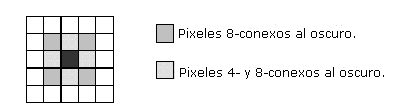
\includegraphics[scale=0.6]{figuras/48conexos.png}
\end{center}
  \caption{\small Tipos de conectividad entre pixeles de una imagen binaria}
  \label{fig:conectividad}
\end{figure}

\begin{figure}[tpb]
\begin{center}
  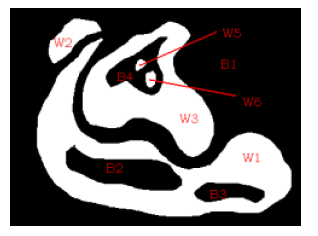
\includegraphics[scale=0.6]{figuras/zonas-contours.png}
\end{center}
  \caption{\small Ejemplo de segmentación en imágenes binarias. Las 1-componentes w1,w2 y w3 se encuentran rodeadas por la componente de fondo b1 y a su vez
  rodean a 0-componentes b2,b3 y b4 }
  \label{fig:contours}
\end{figure}
	
	
	\paragraph{Representación}
	Como se expresa en el trabajo de Zhang y Lu \cite{Zhang02}, existen diversas formas de representar los contornos, cada una con
	distintas aplicaciones. En nuestro caso se utilizan la codificación encadenada de Freeman, que consiste describir una sucesión de puntos
	de acuerdo a la posición de un punto con respecto a su predecesor en la secuencia. Para esto se númeran los vecinos de un pixel con 
	los números del 1 al 7 como indica la figura \ref{fig:freeman}. De esta manera, un contorno puede almacenarse como la coordenada de
	un punto inicial seguido de una cadena de códigos (del 1 al 7) que indican la posición del próximo punto respecto al actual. Esta 
	es una representación más compacta en comparación con una secuencia 
	de coordenadas  $(x,y)$ y posibilita la extracción de 
	caracteristicas tales como el CCH o NCCH \footnote{ CCH o chain 
	code histogram es un histograma que se extrae a partir de la 
	frecuencia de aparición de los números 1 a 7 en un contorno 
	codificado con cadenas de Freeman. Este descriptor es invariante 
	frente a traslaciones y escalamientos pero no frente a rotaciones 
	para lo que existe su versión normalizada NCCH. Para más detalle 
	ver \cite{Iivarinen96shaperecognition}}. La figura \ref{fig:freeman_sample} exhibe un 
	ejemplo de codificación utilizando este método.
	
	\begin{figure}[htpb]
\begin{center}
  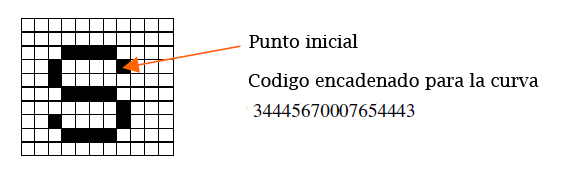
\includegraphics[scale=0.6]{figuras/freeman-sample.png}
\end{center}	
  \caption{\small Ejemplo de codificación de un contorno utilizando los códigos de Freeman. }
  \label{fig:freeman_sample}
\end{figure}

\begin{figure}[htpb]
\begin{center}
  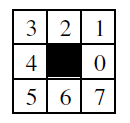
\includegraphics[scale=0.6]{figuras/freeman-codes.png}
\end{center}
  \caption{\small Matriz para la codificación de freeman. El número indica la dirección de desplazamiento del próximo punto respecto del
  actual (punto negro) }.
  \label{fig:freeman}
\end{figure}
		
		
	\paragraph{Polígonos}
	Como mencionamos, los contornos son representados utilizando la codificación de Freeman. Sin embargo, la precisión con la que se muestrean estos bordes suele ser excesiva o redundante para nuestras
	necesidades lo cual hace el análisis de figuras más dificil. Con el fin de reducir esta complejidad utilizamos un algoritmo
	para representar el mismo contorno con una menor cantidad de puntos. Esto se realiza mediante un algoritmo de aproximación por polígonos
	basado en el trabajo de Douglas y Pecker \cite{dp74}. Previo a la aplicación de este algoritmo, convertimos el contorno a una representación
	tradicional de secuencias de puntos $(x,y)$ correspondientes a las 
	coordenadas del borde en la imagen. Esto se puede lograr facilmente partiendo del punto inicial y calculando la variación en la coordenada según el código de vecino correspondiente ( 0-7).\\
	\indent La técnica de aproximación comienza tomando los dos puntos 
	pertenecientes al contorno mas alejados entre si. Estos puntos se 
	agregan a la aproximación y se traza una línea entre ellos.
	Luego se recorre el resto de los puntos del contorno buscando a aquel 
	que se encuentre a mayor distancia de esta línea. A dicho punto se lo 
	agrega a la aproximación, generando dos nuevas líneas con los dos puntos iniciales. Este proceso se itera agregando siempre el punto que se encuentre mas distante de la aproximación hasta que todos los puntos del contorno se encuentren a una distancia menor que cierto parámetro 
	de precisión establecido. En la figura \ref{fig:polyaprox} podemos apreciar una esquematización de este proceso. Otra ventaja que 
	otorga la utilización de esta aproximación es que si un contorno presenta una serie de puntos alineados, estos serán remplazados por un 
	único segmento o lado del polígono, lo que nos permite identificar lineas en los contornos. Esta caracteristica es aprovechada para
	realizar la detección de vasos como se ve en la próxima sección. En la figura \ref{fig:polyVasos} podemos observar un contorno
	y su aproximación por polígonos.
	
\begin{figure}[htpb]
\begin{center}
  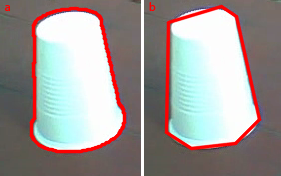
\includegraphics[scale=0.8]{figuras/polyaprox.png}
\end{center}
  \caption{\small Aproximación de contornos mediante polígonos. (a) Se observa que el contorno se encuentra acorde el borde del vaso, las
  partes laterales del mismo se encuentran segmentadas (efecto serrucho) por la cantidad de puntos. (b) El contorno es representado mediante
  8 puntos, los lados laterales solo involucran un segmento posibilitando la detección de lineas.}
  \label{fig:polyVasos}
\end{figure}

\begin{figure}[htpb]
\begin{center}
  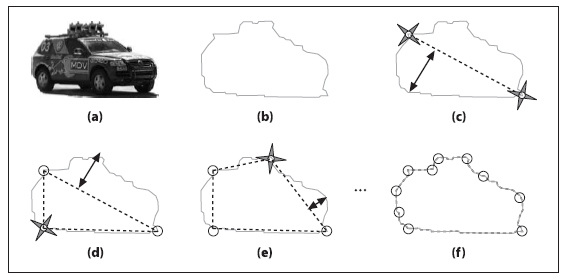
\includegraphics[scale=0.6]{figuras/douglas-pecker.png}
\end{center}
  \caption{\small Iteraciones del algoritmo de aproximación de polígonos de Douglas-Peucker. (a) Imagen original. (b) Extracción de contorno
  (c) Se seleccionan dos puntos iniciales y se traza una línea entre ellos (d) Se agrega a la aproximación el punto mas lejano del contorno a esta línea.
  (e) Se repite el proceso agregando siempre el punto mas lejano (f) hasta que todos los puntos esten a cierta distancia requerida.}
  \label{fig:polyaprox}
\end{figure}

	

	\subsubsection{Filtros}
	Realizada la etapa de pre-procesamiento y la recolección de contornos de la imagen el paso que sigue es verificar que estos
	contornos tengan características que correspondan con  los 
	objetos buscados. Para realizar esto, se implementan una serie de filtros que verifican propiedades
	puntuales sobre los mismos, si un contorno supera todos los filtros entonces consideramos a tal como un objeto reconocido. \\
	\indent Los filtros se disponen en cascada, es decir, se prueba un filtro en un contorno solo si este superó todos los filtros 
	anteriores. De esta forma podemos ordenar los filtros de más general a más específico, optimizando los tiempos de detección. Por ejemplo , conocer 
	el área que abarca un contorno determina fácil y rápidamente si un contorno corresponde a una colilla o a un plato evitando la ejecución
	de filtros más específicos. A continuación detallamos los filtros realizados:
	\paragraph{Filtro de área}
	El filtro de área calcula el área encerrada por un contorno y verifica que la misma se encuentre por encima y/o por debajo
	de valores determinados. El área encerrada por un contorno se computa utilizando la formula de Green \cite{greenwolfram}.
	Si bien esto es más veloz que contabilizar todos los pixeles encerrados en el contorno, posee la desventaja que no se tienen en cuenta agujeros
	en el interior del mismo.
	\paragraph{Filtro de área por zona}
	Un objeto que posee un área determinada puede ocupar más o menos pixeles dependiendo de su ubicación en la imagen. Este se debe a la 
	perspectiva de la cámara y puede afectar al reconocimiento de un contorno. Para contemplar esta variación se pueden establecer distintas
	zonas en la imagen y definir distintos valores de área mínimos y máximo para cada una de ellas. Al ejecutarse este filtro se calcula la
	zona a la cual pertenece dependiendo de su ubicación en la imagen y se verifican los valores para dicha zona, si este los satisface entonces
	el contorno supera al filtro.
	\paragraph{Filtro de perímetro}
	El filtro de perímetro calcula , efectivamente, el perímetro cubierto por un contorno. Esto se hace contando la cantidad de pixeles que lo definen.
	Vale remarcar, que el valor del perímetro depende ampliamente de la precisión con la que se obtengan los bordes ya que se ve drásticamente modificado 
	si se aumenta o disminuye dicha precisión.
	\paragraph{Filtro de excentricidad}
	La excentricidad es un parámetro que relaciona la longitud del eje más largo con el del más corto. Esta se define como 
	\textit { longitud del eje mas largo / longitud del eje mas corto}  . Algunas figuras pueden caracterizarse por tener valores de excentricidad
	que se mantienen en cierto rango y permite identificarlas usando este filtro.
	\paragraph{Filtro de circularidad}
	La circularidad es un parámetro que relaciona área con perímetro y define la redondez de una figura. Se define como $perimetro^2/area$. Algunas figuras pueden 
	caracterizarse por tener valores de circularidad que se mantienen en cierto rango y permite identificarlas usando este filtro.
	\paragraph{Filtro de área rectangular}
	El filtro de área rectangular relaciona el área del objeto con el área del rectángulo contenedor mínimo. Este verifica que el área
	del contorno cubra en gran parte el área del rectángulo. Esto se logra mediante la división $(area contorno / area rectangulo)> p$, donde 
	$p$ es el porcentaje de área que queremos que sea cubierto.
	\paragraph{Filtro de elipse}
	El filtro de elipse verifica que un contorno determinado se ajuste o no a una elipse. Esto se logra usando un algoritmo basado 
	en cuadrados mínimos. El mismo retorna como resultado las longitudes de los semi-ejes de la elipse $a$ y $b$. Con estas medidas calculamos
	el área según la fórmula $A=\pi a  b$ y se la compara con la 
	obtenida a través del filtro de área. Se computa como $|A-AReal|/ 
	AReal < p$ donde p determina el
	valor de verosimilitud, donde más chico significa más parecido. Si estas dos áreas son lo suficientemente similares consideramos que el contorno supera el filtro. 
	Para el ajuste de elipse se utiliza el algoritmo Fitzgibbon, Pilu y Fisher \cite{Fitzgibbon99}.
	\paragraph{Filtro de vaso}
	El filtro para vasos consiste en varias etapas. Recordando que el contorno se codifica como un polígono, se obtienen los dos segmentos 
	más largos y se verifica que estos no compartan vértices. Por otro lado se pide que la suma de la longitud de estos dos segmentos supere al $50\%$ del 
	perímetro del contorno, indicado por dicho filtro. Finalmente, se verifica que la distancia mínima entre estos dos ejes sea mayor a cierto valor prefijado, proporcional a la
	longitud del segmento más largo. El filtro se basa en la idea de que 
	los dos segmentos más largos se correspondan con los lados laterales 
	del vaso.  Se puede apreciar una foto  de un contorno que ha 
	verificado este filtro en la figura \ref{fig:polyVasos}. 
	\paragraph{Filtro de histograma}
	El filtro de histograma verifica la similitud de un histograma obtenido a partir del contorno con otro histograma obtenido a partir de 
	una imagen modelo del objeto a detectar. El histograma modelo se calcula en el inicio de la ejecución mientras que el del contorno se
	computa en tiempo real. Esto se hace obteniendo el rectángulo contenedor mínimo de dicho contorno y computando un histograma 2d de la imagen
	utilizando los canales de saturación y tono. Esto permite caracterizar a un objeto por una composición de colores y no por su forma. El 
	problema de este filtro es que requiere mayor procesamiento.
	
	\subsubsection{Reconocimiento de vasos}
	Para el reconocimiento de vasos se utilizan(en este orden) los filtros de área, perímetro, circularidad y el de vasos.
	El filtro de área verifica que $500 \leq area \leq 10000 $ , el de perímetro que $100 \leq per \leq 800 $ , el de circularidad
	que $14 \leq circ \leq 18$. El filtro de vasos no es parametrizado. 
	
	\subsubsection{Reconocimiento de colillas}
	Para el reconocimiento de vasos se utilizan(en este orden) los filtros de área, perímetro y área rectangular.
	El filtro de área verifica que $50 \leq area \leq 800 $, el de perímetro que $10 \leq per \leq 150 $ y el de área rectangular
	que sea cubierto el $70\%$ del área del rectángulo contenedor mínimo.
	
	\subsubsection{Reconocimiento de platos}
	Para el reconocimiento de platos se utilizan(en este orden) los filtros de área, perímetro, circularidad, excentricidad y de elipse.
	El filtro de área verifica que $500 \leq area \leq 10000 $ , el de perímetro que $500 \leq per \leq 1500 $ , el de circularidad
	que $10 \leq circ \leq 16$, el de excentricidad que $0.65 \leq ecc \leq 0.95$ y el de elipse que $|a-aReal|/ aReal < 0.2$.
	
	\subsubsection{Centroide}
	En las siguientes secciones se hacen referencia a los centroides 
	de un objeto. El centroide es el centro geometrico o centro de 
	gravedad de una figura y 
	sirve como punto de referencia para la misma. Para calcular dicho 
	punto hacemos uso de las formulas propuestas por Hu \cite{Hu1962} para la 
	descripción de figuras. El momento de Hu de un contorno 2d se define como:
	\begin{equation}
		m_{pq}=\sum_{x}{\sum_{y}{x^py^qI(x,y)}}
	\end{equation}
	
	donde $I(x,y)$ es la intensidad del pixel de coordenadas $(x,y)$.
	Notamos que $m_{0,0}$ representa la suma de la intensidad de todos los pixeles del 
	contorno. Entonces, podemos definir al centroide $(x_c,y_c)$ como 
	$x_c= m_{1,0} / m_{0,0}$ e 
	$y_c=m_{0,1} / m_{0,0}$. Estas dos fórmulas se corresponden con el 
	promedio de las coordenadas x e y de los puntos de la figura.  


\begin{figure}[tpb]
\begin{center}
  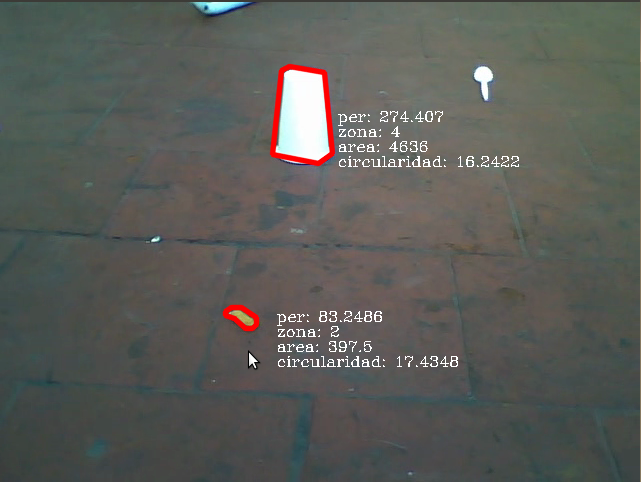
\includegraphics[scale=0.4]{figuras/filtros.png}
\end{center}
  \caption{\small Ejemplo de descriptores de contorno. Se visualiza el área, perímetro, zona y circularidad del contorno 
  detectado de una colilla y un vaso}
  \label{fig:erode}
\end{figure}

	\subsection{Sistema de predicción}
	El algoritmo de visión que hemos descripto hasta aquí funciona 
	procesando la imagen correspondiente a un único cuadro. Sin embargo, 
	el sistema de visión del robot debe permitir el reconocimiento de 
	objetos a medida que esta se desplaza por su entorno y por lo tanto 
	dicho sistema debe procesar imágenes secuenciales del mismo. Con 
	esto afirmamos que existe cierta relación entre las imágenes 
	que el sistema de visión debe procesar y que podemos aprovechar esta 
	característica para reforzar la detección de objetos.  El mecanismo por el cual buscamos lograr este objetivo es el del sistema de predicción.\\
\indent 	El sistema de predicción consume la información que el 
sistema de visión le entrega en cada cuadro y, con ella, realiza el 
seguimiento de objetos a lo largo del tiempo. Es a partir de este 
seguimiento que el sistema de predicción toma decisiones sobre la 
posición o existencia de los objetos que el sistema de visión 
reconoce. Vale destacar que estos dos sistemas pueden encontrarse, a 
menudo, en desacuerdo acerca de presencia u ausencia 
de un objeto.  El sistema de predicción se basa en las siguientes asunciones:
\begin{enumerate}
\item{ Los objetos no realizaran grandes desplazamientos entre cuadros 
consecutivos - esto se debe la proximidad temporal entre cuadros y que el robot no realiza movimientos bruscos.}
\item{ Los objetos no sufrirán grandes alteraciones en su forma, área 
o perímetro entre cuadros consecutivos - con un razonamiento similar, la perspectiva no cambia lo suficiente como para alterar la figura, área o perímetro de los objetos.}
\end{enumerate} 
Con estas premisas, dado un objeto $A$ reconocido en el cuadro $c_0$, 
cuyo centroide se encuentra en las coordenadas (en la imagen) $(x_0,y_0)$, área $a$ y perímetro $p$, 
el sistema de predicción asume que si se encuentra un objeto $A'$ en 
el cuadro siguiente $c_1$ con coordenadas $(x_1, y_1)$ tal que 
$||(x_1,y_1) - (x_0,y_0)||\leq \alpha$, área $a'$ tal que $|a-a'| \leq 
\gamma *a$ y perímetro $p'$ tal que $|p-p'|\leq \theta*p$ entonces $A 
\simeq A'$, donde $\alpha$, $\gamma$ y $\theta$ son parametros del 
sistema. Esta aseveración no solo vale para el cuadro subsiguiente 
$c_1$ sino también para los siguientes $c_2,c_3 ... c_{0+\eta}$ donde 
$\eta$, $\alpha$ y $\gamma$ se computan, para este caso, según el 
historial de detección de cada objeto.  Basandose en esta regla, el 
sistema de predicción puede estimar la posición de un objeto que, 
para un cuadro en particular, no fue detectado por el sistema de 
visión. Para concretar este mecanismo, cuando un objeto es detectado a lo largo de varios cuadros se persiste la siguiente información:
\begin{itemize}
\item{ Última posición, área y perímetro - Se toman los datos de la detección mas reciente del sistema de visión .}
\item{ Antigüedad del objeto - Cantidad de cuadros transcurridos desde que se comenzó a persistir el objeto en el sistema de predicción.}
\item{ Cantidad de detecciones - Se mantiene la cantidad de cuadros en la cual el sistema de visión detectó al objeto.}
\item{ Desplazamiento en la posición - Si el objeto es detectado más 
de una vez, se almacena el último desplazamiento en la posición $(x_i - 
x_{i-1} , y_i - y_{i-1} )$.}
\item{ Antigüedad de la última detección - Cantidad de cuadros que transcurrieron desde la última detección por parte del sistema de visión.}  
\end{itemize}
Esta información no solo nos permite corregir al sistema de visión 
cuando este no detecta un objeto sino que también podemos corregirlo 
cuando este no rechaza falsas detecciones de objetos inexistentes. Para 
implementar estos mecanismos se establecen las siguientes reglas sobre 
la persistencia de objetos:
\begin{enumerate}
\item{Un objeto debe ser detectado por el sistema de visión en $\delta$ 
cuadros consecutivos para ser considerado como tal por el sistema de 
predicción}
\item{El sistema de predicción descarta un objeto considerado si el 
sistema de visión no lo detecta en un número $\eta$ de cuadros 
consecutivos.}
\item{ $\eta$ se calcula cada $\lambda$ cuadros como 
$\frac{detecciones}{antiguedad}\times \rho$ donde $\rho$ es un parámetro del 
sistema}.
\item{ Si un objeto es considerado por el sistema de predicción y este 
no es detectado por el sistema de visión para algún cuadro entonces 
el sistema de visión realiza una estimación de su posición de 
acuerdo a la información persistida a partir de sus apariciones en cuadros anteriores.}
\end{enumerate}

Estas reglas, aunque parezcan complejas por el número de variables que 
manejan, son realmente intuitivas. El sistema de predicción consume la 
información que el sistema de visión le brinda y la manipula con 
cierta desconfianza de acuerdo a su 
conveniencia. En una primera instancia, los objetos deben ganarse la 
confianza del sistema de predicción apareciendo \footnote{Con 
aparición nos referimos a que el objeto sea reconocido por el sistema 
de visión.} regularmente en 
cuadros consecutivos, en concordancia con la asunción número 
1. De no cumplir con esta asunción, consideramos que no se trata de un 
objeto de interes e utilizamos la regla 1 para eliminar dicha detección. \\
	Una vez ganada la confianza del sistema de predicción, este 
	último comienza a tener a estos objetos en consideración 
	\footnote{Decimos que el sistema de predicción considera a un 
	objeto cuando este empieza a informar la posición de este dentro de la 
	imagen. Notese que, para un cuadro determinado, el sistema de 
	visión puede detectar un objeto y el sistema de predicción, como 
	todavía no considera a dicho objeto, ignora la detección y no informa de su 
	presencia.} y veta por su 
existencia aunque el sistema de visión no los detecte. El grado en que 
el sistema cree en la existencia de estos objetos se va regulando de 
acuerdo al historial de apariciones de los mismos. Si estos abusan de 
la confianza otorgada entonces el sistema de predicción los descarta 
como indica la regla 2. 
Este grado de confianza o de libertad se traduce en cantidad de 
cuadros que puede pasar un objeto sin ser detectado por el sistema de 
visión y siendo considerado por el sistema de predicción. Dicho 
número se determina periódicamente utilizando la fórmula de la regla 3.
Finalmente, durante este lapso de confianza, el sistema de predicción 
'aproxima' la posición de los objetos si estos no son detectados por el 
sistema de visión, como dice la regla 4. \\
\indent La variable $\alpha$ determina la distancia máxima que puede 
desplazarse un objeto entre cuadros para que el sistema de predicción lo considere 
como el mismo. Las variables $\gamma$ y $\theta$ determinan el máximo 
porcentaje de variación en el área y perímetro que puede soportar un 
objeto entre cuadros para ser considerado como el mismo. Valores 
típicos para la detección de colillas y vasos son de 
$0.1\leq\gamma\leq0.3$ y $0.1\leq\theta\leq0.3$. Para el caso de 
$\alpha$ definimos un valor aproximado de 30 pixeles. Sin embargo, la 
tolerancia en el desplazamiento varía según los cuadros transcurridos desde la última 
detección. Si en el cuadro anterior fue detectado entonces se utiliza 
$\alpha$ , si fue detectado hace dos cuadros entonces $2\alpha$, tres 
cuadros $3\alpha$ y así. La variable $\delta$ establece el umbral de 
detección de un objeto por parte del sistema de visión para que el 
sistema de predicción lo empiece  a considerar. $\rho$ establece, 
independientemente de la  
regularidad de un objeto, la cantidad máxima de cuadros que puede 
permanecer este sin ser detectado por el sistema de visión y 
considerado por el sistema de predicción. \\ 
\indent Es importante destacar que tanto $\rho$ como $\delta$ repercuten directamente en la 
performance de detección. En el caso de la variable $\delta$, el 
sistema de visión debe reconocer un objeto $\delta -1$ veces antes de que sea 
tenido en consideración por el sistema de predicción y, en este lapso, las 
detecciones serán ignoradas. Sin embargo, las apariciones no sostenidas 
(de hasta $\delta -1$ cuadros) de elementos que aparentan ser objetos 
para el sistema de visión pero no lo son, son también ignoradas, 
disminuyendo el porcentaje de falsos negativos.\\
\indent La variable $\rho$, en cambio, establece otro tipo de balance. 
	Siempre que un objeto deja de aparecer en la imagen (por 
	desplazamiento del objeto o del robot), el sistema de 
	predicción arriesga la posición de este un máximo de $\rho$ veces 
	(según la regularidad de detección) y, en esta caso, las equivoca a 
	todas ya que el objeto no figura más en la imagen. El lado 
	positivo es que cuando un objeto que tenía un historial de 
	detección positivo es ocluido o alterado de tal forma que el 
	sistema de visión no lo reconoce, el sistema de predicción 
	arriesgará la posición (hasta $\rho$ veces) pudiéndole acertar o no hasta que el objeto 
	sea nuevamente detectado por el sistema de visión o sea descartado. 
	Es en esta última situación es donde se obtienen nuevas detecciones que el sistema de visión 
	nunca podría obtener por sí solo.\\
	\indent A partir de estas reflexiones surge la importancia de configurar 
	estas variables de acuerdo al sistema de visión que estemos 
	usando. Si tenemos un sistema de visión con alto porcentaje de 
	falsos positivos y bajo porcentaje de falsos negativos entonces es 
	probable que arriesgar más posiciones de objetos cuando estos no 
	son detectados mejore la performance. En este caso debemos elegir 
	valores de $\rho$,no muy pequeños, para afrontar el déficit de 
	detección del sistema de visión  y valores de $delta$,mas bien 
	pequeños, para no entorpecer la detección. Es importante remarcar 
	que el bajo porcentaje de falsos positivos, en este caso, nos 
	permite confiar en el sistema de visión en el sentido de que las cosas que 
	este detecte tienen altas probabilidades de ser objetos. \\
	\indent En el caso reciproco, un sistema de visión con alto 
	porcentaje de falsos negativos y bajo porcentaje de falsos 
	positivos quizás convenga tener un valor de $\delta$ alto, para 
	filtrar la mayor cantidad de detecciones falsas. Al hacerlo, puede 
	suceder que también filtremos detecciones positivas pero en ese 
	caso habría que estudiar cuanto se gana y cuanto se pierde y 
	buscar un balance.\\
	\indent Otra posibilidad es que el sistema de visión sea muy 
	confiable ( bajo porcentaje de falsos positivos/negativos). En 
	esta situación conviene configurar al sistema de predicción para 
	que haga más caso de lo que el sistema de visión le informa. Esto 
	significa que cuando el sistema de visión no encuentra un objeto 
	el sistema de predicción no debe arriesgar mucho ya que el objeto 
	probablemente no se encuentre. Asimismo, unas pocas detecciones de 
	un objeto bastan para que el sistema de predicción lo tenga 
	en consideración ya que existe una alta probabilidad de que 
	realmente se trate de un objeto. Esto se traduce en valores de 
	$\delta$ y $\rho$ bajos.
 


  %~ La regla 1 nos permite eliminar las detecciones 
%~ espontáneas de objetos por parte del sistema de visión. Si observamos nuevamente la 
%~ asunción número 1, entonces no está mal decir que un objeto que 
%~ fue detectado en un cuadro determinado debería aparecer(con cierta 
%~ probabilidad) en los subsiguientes. Bajo 
%~ este criterio utilizamos la regla 1 para descartar a aquellos objetos 
%~ que no cumplen con dicha proposición. En cambio, si el objeto es detectado de forma 
%~ regular en un número de cuadros estipulados, entonces el sistema de 
%~ predicción da fe de la existencia de ese objeto otorgándole la 
%~ posibilidad de no ser detectado por el sistema de visión por un 
%~ número determinado de cuadros. En este caso, el sistema de predicción 
%~ veta por la existencia del objeto ya que dispone de una muestra 
%~ suficiente para creer eso.  Esta creencia se mantiene por un número de 
%~ cuadros que se calcula de acuerdo al grado de regularidad en el que fue 
%~ detectado anteriormente. Para ejemplificar, un objeto que apareció en 10 de los últimos 12 
%~ cuadros podrá permanecer mas cuadros sin ser detectado por el sistema 
%~ de visión y, sin ser descartado por el de predicción, que otro objeto 
%~ que solo apareció en 5 de los últimos 12 cuadros. Cuando se agota la 
%~ cantidad de cuadros que un objeto puede no ser detectado, el sistema 
%~ de predicción lo descarta. 
%~ . 

	\subsection{Focalización}
	Focalización es el mecanismo que busca que el sistema de visión se 
	concentre en la detección de un único objeto a lo largo del tiempo. 
	Esta situación es deseable cuando el sistema de visión ya detectó 
	una basura y el robot se dirige a recolectarla. En esta circunstancia, 
	no nos interesan otros objetos que puedan aparecer durante el trayecto 
	y por lo tanto tratamos de evitar cualquier tipo de procesamiento 
	innecesario sobre ellos. Con este objetivo, seleccionamos una 
	sub-imagen a procesar en la cual suponemos que vamos a encontrar al 
	objeto en cuestión. El mecanismo de focalización se encuentra muy 
	ligado al sistema de predicción ya que debe persistir cierta 
	información sobre la posición del objeto para poder tomar una 
	sub-imagen que lo contenga.\\
\indent El mecanismo de focalización puede separarse en dos etapas. En una primera etapa, utilizando la información brindada por el sistema de predicción, se selecciona un objeto a focalizar. Existen varios criterios de selección, algunos que consideramos más relevantes son:
\begin{itemize}
\item{ Objeto más cercano - Se estiman las distancias a los objetos y se selecciona aquel que se encuentre más cercano al robot.}
\item{ Objeto más detectado en los últimos 20 cuadros - Se selecciona al objeto que fue reconocido más veces por el sistema de visión en las últimas 20 imágenes.}
\item{ Objeto más antiguo - Se elige al objeto que persistieron más cuadros según el sistema de predicción.}
\item{ Combinación ponderada - Se utilizan los  criterios mencionados dándoles mayor o menor peso a cada uno y eligiendo al objeto que obtenga mayor puntuación.}
\end{itemize}
Pensamos todos los criterios con el objetivo de maximizar las chances 
de que el robot tenga éxito en la recolección del objeto. El criterio de menor distancia implica un menor recorrido hacia el objeto y por lo tanto menos posibilidades de cometer error durante el recorrido. Si utilizamos el criterio de mayor detección en los últimos 20 cuadros estamos maximizando las chances de que el sistema de visión detecte al objeto durante el trayecto del robot hacia el mismo. Con un razonamiento similar, el criterio de mayor antigüedad maximiza las chances de que el sistema de visión detecte al objeto pero utilizando información más general y no tan local como el resultado de los últimos cuadros. Previo a la focalización es necesario alimentar al sistema de predicción ya que sin este, no es posible utilizar ninguno de los criterios mencionados.\\ 
	\indent Una vez que seleccionamos el objeto, utilizamos el sistema de 
	predicción para dar cuenta de la posición del mismo. Con esta 
	información, tomamos sub-imágenes (ventanas) de la captura original 
	que solo abarquen un entorno del objeto como se aprecia en la figura 
	\ref{fig:ventaneo} y \ref{fig:ventaneo_2} . Esto provoca una 
	disminución en el tiempo de procesamiento requerido ya que solo se procesa una fracción de 
	la imagen. El tamaño de la ventana queda determinado por 
	las dimensiones del contorno del objeto a focalizar. Si consideramos 
	al sistema de visión como un sensor podríamos decir que este 
	mecanismo incrementa la frecuencia de muestreo del mismo ya que 
	permite tomar una mayor cantidad de muestras en menor tiempo. La 
	focalización sobre un objeto finaliza únicamente cuando este objeto 
	deja de ser reconocido por el sistema de predicción y entonces 
	retomamos al  procesamiento de la imagen completa donde se 
	seleccionara un nuevo objeto a focalizar. 

\begin{figure}[htpb]
\begin{center}
  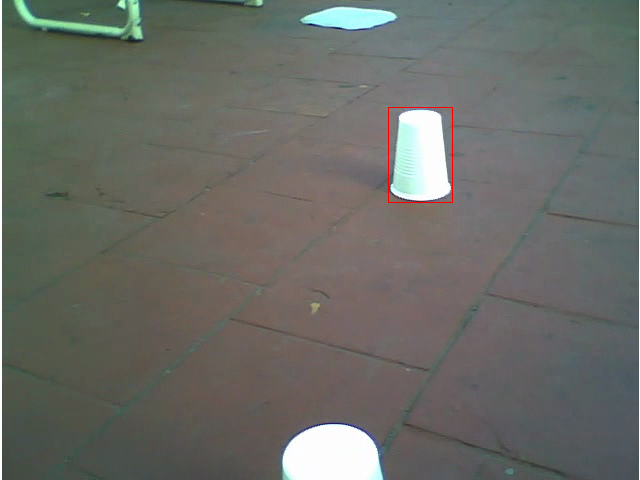
\includegraphics[scale=0.4]{figuras/ventana-1.png}
\end{center}
  \caption{\small Se observa un vaso delimitado por un rectángulo 
  contenedor mínimo rojo. El rectángulo se utiliza para calcular el 
  tamaño de la sub-imagen previo al ventaneo.}
  \label{fig:ventaneo}
\end{figure}


\begin{figure}[htpb]
\begin{center}
  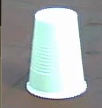
\includegraphics[scale=0.6]{figuras/ventana-2.png}
\end{center}
  \caption{\small Ventana o sub-imagen obtenida de un vaso en 
  focalización. El tamaño de la ventana es de tamaño proporcional al 
  contorno del objeto en cuestión.}
  \label{fig:ventaneo_2}
\end{figure}

	
	
\subsection{Resultados}
En esta sección se describen los parámetros utilizados para la 
medición de la performance y se muestran los resultados obtenidos para 
el sistema de visión y un sistema de visión con predicción. De este 
últimos exhibimos dos configuraciones. Tomamos 8 videos de prueba en los cuales 3 pertenecen a 
colillas, 3 a vasos y 2 a platos. Los videos fueron tomados utilizando 
una silla de oficina giratoria para poder desplazarse suavemente por 
el entorno simulando el movimiento del robot. La cámara se ubicó a 30 
cm del piso formando un ángulo de $30^{\circ}$ con el asiento  en dirección 
hacia el suelo. La cámara utilizada es una microsoft lifecam vx-700 del tipo webcam y posee una 
resolución de 640x480.

\subsubsection{Parámetros de medición}
Con el objetivo de  medir la efectividad del algoritmo de detección, desarrollamos un sistema de benchmarking. Este sistema permite
a un usuario indicar la presencia de objetos a detectar en un video, marcándolos con rectángulos en las sucesiones de cuadros. De esta
manera, corremos el algoritmo de detección por el mismo video y verificamos que los centroides de los objetos detectados por el algoritmo 
se encuentren contenidos dentro de los rectángulos indicados por el 
usuario. Para obtener estadísticas sobre la performance  
medimos los siguientes parámetros:
\begin{itemize}
\item { Cantidad de objetos a detectar \textbf{(\#O)}: Se corresponde con la cantidad de rectángulos marcados por el usuario}
\item { Hits\textbf{(H)} : Cantidad de detecciones por parte del algoritmo que se corresponden con rectángulos marcados.}
\item { Misses o detecciones falsas \textbf{(M)} : Cantidad de detecciones por parte del algoritmo que no se corresponden con rectángulos marcados.}
\end{itemize}
Se desprende directamente que la cantidad de detecciones: 
\textbf{$\#D=H+M$} .
Con estos datos obtenemos los porcentajes de error , falsos positivos : 
\[
	fp=1 - \frac{H}{\# O}
\]
y falsos negativos:
\[
	fn=\frac{M}{\# D}
\]
En el caso óptimo, ambas medidas de error tendrán un valor de $0\%$.  \\
\indent A estas estadísticas se agregan las particulares para el sistema de predicción. Recolectamos información sobre
cuántos casos el sistema de predicción estimó la posición y acertó . Denominamos
a la cantidad de estimaciones realizada por el sistema de predicción 
con \textbf{G} mientras que a las estimaciones que además fueron 
acertadas \textbf{G\&H}.

\subsubsection{Análisis}
Exhibimos los resultados obtenidos tras utilizar solo el sistema de 
visión en el cuadro \ref{tab:result} e utilizando el sistema de 
visión con el sistema de predicción, utilizando dos configuraciones 
distintas, en 
los cuadros \ref{tab:pred} y  \ref{tab:pred_2}. Además exhibimos los 
resultados promedios de falsos positivos y falsos negativos agrupados 
por objeto para todas las configuraciones en los cuadros \ref{tab:evo_colillas}, 
\ref{tab:evo_vasos} y \ref{tab:evo_platos}. Las configuraciones 
utilizadas fueron seleccionadas para destacar distintos comportamientos del 
sistema de predicción, estas son:
\begin{itemize}
\item{\textbf{Configuración 1:} $\lambda=10$, $\rho=10$, $\delta=3$}
	\item{\textbf{Configuración 2:} $\lambda=10$, $\rho=4$, $\delta=2$}
\end{itemize}
\indent En los resultados arrojados en el cuadro \ref{tab:result} solo por el sistema de visión 
observamos problemas en la  detección de colillas ya que posee altos 
porcentajes de falsos negativos. Esto indica que el detector, en el 
caso de las colillas, tiene
problemas en distinguir a estas de su entorno ya que comete 
demasiados errores al reconocer colillas que no existen. Esto concuerda 
con el hecho de que, en el caso de las colillas, el número de 
detecciones \#D es siempre mayor que \#O también observado en el 
cuadro \ref{tab:result}. No obstante, al utilizar el sistema de 
predicción observamos una gran reducción de este porcentaje producto 
del filtrado realizado por dicho sistema el cual no considera una 
basura hasta que esta se presente en $\delta$ cuadros consecutivos.  
Esta mejora viene acompañada de efecto negativos ya que la cantidad de 
hits se ve afectada pero con menor intensidad. Esto prueba que el 
filtrado realizado es efectivo ya que elimina, sobre el total de las 
detecciones, en mayor proporción a 
aquellas que son falsas. El cuadro \ref{tab:evo_colillas} exhibe las ventajas de utilizar un sistema de 
predicción para las colillas.\\
\indent 
En el caso de los vasos, observamos que el sistema de visión brinda 
una muy buena performance por si solo, como se ve en el cuadro \ref{tab:result} 
donde se muestran valores menores al $10\%$ en falsos positivos y falsos 
negativos para todos los videos. La diferencia de performance con la 
detección de colillas es comprensible ya que los vasos poseen 
caracteristicas como tamaño y color que hacen que sea más facil 
reconocerlos y mas dificil confundirlos en relación con estas 
últimas, que poseen un color similar al del fondo y son de tamaño 
pequeño. En este caso, el sistema de predicción no altera demasiado 
los resultados como en el caso de las colillas, sin embargo, destacamos un 
aumento en la cantidad de detecciones falsas en la configuración 1 
,atribuido a el valor elevado de $\rho$, acompañado de un incremento 
similar en el porcentaje de aciertos. Distinto es el caso de 
la configuración 2 que disminuye levemente el porcentaje de falsas 
detecciones y el porcentaje de aciertos respecto de los resultados
obtenidos por el sistema de visión. El comportamiento de la 
configuración 2 es razonable ya que esta es una configuración menos 
invasiva y más respetuosa del sistema de visión subyacente en 
comparación con la configuración 1. Esto se ve reflejado, en parte, 
en la cantidad de estimaciones ( \textbf{G} ) y estimaciones correctas 
(\textbf{G\&H}) cometidas por cada configuración. Podemos 
apreciar las diferencias entre las distintas configuraciones para los 
vasos en el cuadro \ref{tab:evo_vasos}.\\
\indent El caso de los platos es similar al de los vasos. El sistema de visión 
obtiene buenos resultados por si solo pero se ve perjudicado por la configuración 1 del sistema de 
predicción ya que este no acierta en gran proporción de las estimaciones que realiza. 
Sin embargo, en este caso , el aumento en el porcentaje de detecciones 
falsas es relativamente mayor que el aumento de aciertos. 
La configuración 2, por otro lado, aumenta el 
porcentaje de aciertos y disminuye la cantidad de detecciones falsas 
aunque en ambos casos, de manera leve, mejorando apenas los resultados 
obtenidos por el sistema de visión. En este caso, los porcentajes de 
aciertos de las estimaciones son bajos pero observamos que utilizando 
la configuración 2 el número de estimaciones es mucho menor con lo 
que se cometen menos errores. Un cuadro comparativo de las 
distintas configuraciónes para vasos pueden observarse en el cuadro 
\ref{tab:evo_platos}.\\
\indent  Las dos configuraciones del sistema de predicción modifican de 
distintas manera al algoritmo de visión subyacente. Para cada objeto 
hemos obtenido resultados y comportamiento particulares lo que 
justifica la necesidad de ajustar los parámetros del mismo para obtener la mejor 
performance posible. Para poder realizar este ajuste es necesario 
establecer que grado de incidencia tienen los dos tipos de errores en la performance del
algoritmo. Por ejemplo, bajo distintas circunstancias podemos preferir que el  
sistema de visión cometa más errores de tipo I (falsos positivos) con 
el objetivo de minimizar errores de tipo II ( falsos negativos) o 
viceversa. En ese sentido el sistema de predicción proporciona los mecanismos que 
permiten lograr estos ajustes sin necesidad de modificar el algoritmo de detección 
subyacente. En nuestro caso consideramos que tal y tal cosa es mas 
importante sobre tal otra por tal y tal motivo como hemos discutido en 
la sección GUILLE.
 

%~ Esto se lo atribuimos a que esta configuración tiene un valor de 
%~ $\rho$ elevado y por lo tanto modifica demasiado la performance del 
%~ sistema de visión. Recordemos que a valores de $\rho$ mas elevados, 
%~ mayor serán el número de estimaciones de la posición de los objetos 
%~ siendo mas propenso a cometer errores. En el caso de los vasos, debido 
%~ a la alta efectividad del sistema de visión, resulta contra-producente  
%~ arriesgar tanto. Esto se verifica utilizando la configuración 2 donde 
%~ ,al realizar una menor cantidad de estimaciones, se obtiene un número mucho 
%~ menor de detecciones falsas sin comprometer tanto la cantidad de 
%~ aciertos. 
%~ caso de los vasos y platos que presentan porcentajes relativamente 
%~ bajos en todos los casos. La diferencia de performance entre los vasos 
%~ y platos con las colillas es esperable ya que las colillas son 
%~ objetos de menor tamaño e incluso poseen un color muy similar al del 
%~ entorno, lo cual dificulta su detección. En cambio, el color blanco y 
%~ el gran tamaño de los vasos y platos hace que se distingan facilmente 
%~ del fondo pero su color los hace mas sensibles a la iluminación.\\
%~ \indent Utilizando el mismo sistema de visión con el sistema de 
%~ predicción  obtenemos resultados un tanto distintos indicados en la 
%~ tabla \ref{tab:pred}. En el caso de las colillas observamos una mejora notable 
%~ en los falsos negativos debido al efecto pasa-altos establecido por 
%~ la variable $\delta$, eliminando las apariciones espontaneas y el 
%~ número de detecciones en general. A su vez, esta disminución impacta 
%~ en la cantidad de hits y por consecuente en el porcentaje de falsos 
%~ negativos, pero de forma mucho mas leve lo que lo hace un trade-off 
%~ favorable. En el caso de los vasos y platos no se observa ninguna 
%~ mejora notoria. En los vasos vemos un leve incremento 
%~ en el porcentaje de falsos positivos producido por $\delta$ pero en 
%~ este caso, a diferencia de las colillas, la disminución en el 
%~ porcentaje de falsos negativos es aún mas pequeña, resultando en un 
%~ balance no favorable. Algo similar sucede con los platos en donde se 
%~ reduce notablemente la cantidad de hits sin ver ninguna mejora en la 
%~ cantidad de detecciones falsas. Esto último puede ser atribuido a la 
%~ gran cantidad de errores cometidos al estimar la posición del objeto 
%~ cuando este no fue detectado por el sistema de visión. En sintesis, el 
%~ sistema de predicción logró una influencia positiva en el detector de colillas
%~ filtrando algunas detecciones falsas pero entorpeció la detección de vasos y platos
%~ donde ya poseíamos una buena performance. La configuración utilizada para el sistema de 
%~ predicción en este cuadro resultó muy invasiva para estos dos detectores y los forzó a 
%~ estimar posiciones de los objetos cuando esto no era necesario ya que se poseia un número bajo de 
%~ deteccions falsas.\\
%~ \indent En el cuadro \ref{tab:pred_2} exhibimos los resultados obtenidos con un sistema de predicción
%~ menos invasivo. En este caso se eligieron valores de $\lambda=10$, $\rho=4$ y $\delta=2$. Tomando un valor
%~ de $\rho$ y $\delta$ le damos mas confianza al sistema de visión como fue explicado previamente. En los vasos y
%~ platos es notable la reducción en la cantidad de falsas detecciones sin afectar demasiado el número de hits logrado.
%~ Esto viene acompañado con el hecho de que el predictor realizo menos estimaciones y aumento su tasa de acierto en todos 
%~ los casos. Los resultados obtenidos para estos dos objetos son mejores que los obtenidos solo con el sistema de visión. 
%~ Sin embargo, en el caso de las colillas, el predictor si impacto en la cantidad de hits por lo que no se observa un 
%~ cambio del todo favorable respecto de la configuración anterior.\\
\begin{table}[htb]
  \begin{tabular}{|l | c | c | c | c | c | c |}
	\hline  
	\textbf{Video} & \textbf{(\#O)} &  \textbf{(\#D)} & \textbf{(H)} & 
	\textbf{(M)} & \textbf{fp} & \textbf{fn}\\
	\hline
	\hline
	vasos1 & 5050 & 4880 & 4849 & 31 & 0.6\% & 3.9\% \\
	vasos3 & 1777 & 1708 & 1696 & 12 & 0.7\% & 4.5\% \\	
	vasos4 & 6196 & 5354 & 5251 & 103 & 1.9\% & 15.2\% \\
	\hline
	colillas1 & 1645 & 1648 & 1282 & 367 & 22.2\% & 22.0\% \\
	colillas2 & 891 & 1045 & 636 &  409 & 39.1\% & 28.6\% \\
	colillas3 & 2708 & 3899 & 2373 & 1526 & 39.2\% & 12.7\% \\
	\hline
	platos1 & 2236 & 1966 & 1832 & 134 & 6.8\% & 18.0\%\\
	platos2 & 1128 & 1228 & 1117 & 111& 9.0\% & 0.9\% \\
	\hline
	\end{tabular}
	\caption{\label{tab:result} Performance del sistema sin el algoritmo de predicción}
\end{table}

%Con predicción
\begin{table}[htb]
  \begin{tabular}{|l | c | c | c | c | c | c | c | c |}
	\hline  
	\textbf{Video} & \textbf{(\#O)} &  \textbf{(\#D)} & \textbf{(H)} & \textbf{(M)} & \textbf{fp} & \textbf{fn} & \textbf{G} & \textbf{G\&H} \\
	\hline
	\hline
	vasos1 & 5050 & 5017 & 4888 & 118 & 2.3\% & 3.2\%  & 245 & 142\\
	vasos3 & 1777 & 1773 & 1707 & 66 & 3.7\% & 3.9\% & 121 & 60 \\
	vasos4 & 6196 & 5703 & 5459 & 240 & 4.2\% & 11.8\% & 536 & 373 \\
	\hline
	colillas1 & 1645 & 1444 & 1330 & 98 & 6.8\% & 19.1\% & 296 & 229 \\
	colillas2 & 891 & 687 & 586 & 95 & 13.9\% & 34.2\% & 127 & 57 \\
	colillas3 & 2708 & 2555 & 2242 & 254 & 10.1\% & 17.2  & 516 & 320\\
	\hline
	platos1 & 2236 & 1966 & 1854 & 218 & 10.5\% & 17.0\% & 179 & 34\\
	platos2 & 1128 & 1228 & 1112 & 167& 13.0\% & 1.4\% & 115 & 16\\
	\hline
	\end{tabular}
	\caption{\label{tab:pred} Performance del sistema con el sistema de predicción para 
	$\lambda=10$, $\rho=10$, $\delta=3$ }
\end{table}

\begin{table}[htb]
  \begin{tabular}{|l | c | c | c | c | c | c | c | c |}
	\hline  
	\textbf{Video} & \textbf{(\#O)} &  \textbf{(\#D)} & \textbf{(H)} & \textbf{(M)} & \textbf{fp} & \textbf{fn} & \textbf{G} & \textbf{G\&H} \\
	\hline
	\hline
	vasos1 & 5050 & 4866 & 4839 & 27 & 0.5\% & 4.1\%  & 83 & 72\\
	vasos3 & 1777 & 1700 & 1689 & 11 & 0.6\% & 4.9\% & 32 & 27 \\
	vasos4 & 6196 & 5318 & 5222 & 96 & 1.8\% & 15.7\% & 241 & 226 \\
	\hline
	colillas1 & 1645 & 1220 & 1168 & 53 & 4.3\% & 28.9\% & 142 & 126 \\
	colillas2 & 891 & 652 & 566 & 86 & 13.1\% & 36.4\% & 78 & 38 \\
	colillas3 & 2708 & 2414 & 2142 & 272 & 11.2\% & 20.0\% & 303 & 158 \\
	\hline
	platos1 & 2236 & 1958 & 1843 & 115 & 5.8\% & 17.5\% & 50 & 16 \\
	platos2 & 1128 & 1211 & 1115 & 96 & 7.9\% & 1.1\% & 26 & 8 \\
	\hline
	\end{tabular}
	\caption{\label{tab:pred_2} Performance del sistema con el sistema de predicción con
	$\lambda=10$, $\rho=4$, $\delta=2$}
\end{table}

\begin{table}[h]
  \begin{tabular}{|l | c | c | c | c | c|}
	\hline  
	\textbf{Configuración} & \textbf{$\bar{fp}$} &  
	\textbf{$\bar{fn}$}& \textbf{G} &  \textbf{G\&H} &  \textbf{G\&H/G} \\
	\hline
	\hline
	Sin predicción  & 18.1\% & 34.9\% & - & - & - \\
	\hline
	Configuración 1 & 20.7\% & 9.5\% & 939 & 606 & 64.5\%  \\
	\hline
	Configuración 2 & 26.0\% & 9.5\% & 523 & 322 & 61.5\% \\
	\hline
	\end{tabular}
	\caption{\label{tab:evo_colillas} Performance promedio de las colillas 
	por configuración y  efectividad de las estimaciones del sistema de predicción}
\end{table}

\begin{table}[h]
  \begin{tabular}{|l | c | c | c | c | c|}
	\hline
	\textbf{Configuración} & \textbf{$\bar{fp}$} &  \textbf{$\bar{fn}$}& \textbf{G} &  \textbf{G\&H} &  \textbf{G\&H/G} \\
	\hline
	\hline
	Sin predicción  & 9.4\% & 1.2\% & - & - & -\\
	\hline
	Configuración 1 & 7.4\% &	3.3\% & 902 & 575 & 63.7\% \\
	\hline
	Configuración 2 & 9.7\% &	1.1\% & 356 & 325 & 91.2\%\\
	\hline
	\end{tabular}
	\caption{\label{tab:evo_vasos} Performance promedio de los vasos según configuración del 
	sistema y efectividad de las estimaciones del sistema de predicción}
\end{table}



\begin{table}[h]
  \begin{tabular}{|l | c | c | c | c | c|}
	\hline
	\textbf{Configuración} & \textbf{$\bar{fp}$} &  \textbf{$\bar{fn}$}& \textbf{G} &  \textbf{G\&H} &  \textbf{G\&H/G} \\
	\hline
	\hline
	Sin predicción &  12.3\% & 7.6\% & - & - & -\\
	\hline
	Configuración 1 & 11.8\% & 12.0\% & 294 & 50 & 17.0\%\\
	\hline
	Configuración 2 & 12.0\% & 6.6\% & 76 & 24 & 31.5\% \\
	\hline
	\end{tabular}
	\caption{\label{tab:evo_platos} Performance promedio de los platos según configuración del 
	sistema y efectividad de las estimaciones del sistema de predicción}
\end{table}



\subsection{Conclusi\'on}
Presentamos un algoritmo para el reconocimiento de distintos objetos en 
un ambiente dinámico en el marco de un robot autónomo capaz de 
recolectar basura. El mismo funciona sobre la librería de visión 
computacional OpenCv y el lenguaje c++.  El algoritmo cuenta
con una etapa de pre-procesado donde se extraen los pixeles de colores de interés y se disminuye el ruido utilizando 
operaciones morfológicas y de threshold. La etapa de procesamiento extrae los contornos y utiliza una aproximación por polígonos
para simplificar el análisis posterior. Este consiste en una serie de 
filtros pre-definidos dispuestos en cascada que interpretan la 
información de contorno y  determinan si se trata 
de un objeto de interes o no. 
Implementamos un mecanismo de predicción parametrizable que funciona 
sobre el algoritmo en cuestión por el cual se puede optimizar la performance de 
detección según las caracteristicas propias de cada detector. Se 
midieron los resultados obtenidos realizando el reconocimiento de 
vasos,colillas y platos obteniendo un promedio de $14\%$ de falsos 
positivos  y $5\%$ de falsos negativos. Finalmente agregamos un mecanismo de focalización por el cual 
el sistema completo puede concentrarse sobre un único objeto reduciendo 
los tiempos de procesamiento. 


\subsubsection{Posibles extensiones}
Existen varios puntos donde consideramos se pude mejorar este sistema 
de visión. Una de las áreas donde se pueden introducir mejoras es en 
la sección de filtros. Como hemos visto, existen novedosas tecnicas de 
descripción y representación de contornos que pueden ser introducidas 
como un filtro adicional sin necesidad de modificar la estructura del 
algoritmo. La utilización de dichas técnicas pueden utiilzarse para 
la caracterización de nuevos objetos a reconocer o bien para reforzar 
los objetos ya tratados. Por otro lado, hallamos al sistema de filtros 
en cascada un tanto limitado para la tarea propuesta ya que frente a 
pequeñas perturbaciones que provoquen que un único filtro rechazo un 
determinado contorno, este último se vera descartado por el sistema. 
Como alternativas a este sistema se puede implementar un sistema de 
votación donde se reúnan los resultados de cada filtro y se tome una 
decisión en base a ellos. Adicionalmente, sería interesante que en 
este sistema de votación se pueda indicar un valor que establezca la 
importancia de cada filtro en relación a un objeto determinado. Otra 
posibilidad, basándonos en el trabajo \cite{potato} expuesto en la 
sección \ref{volunteer}, es utilizar las 
caracteristicas medidas por los filtros para entrenar un clasificador. 
Luego este sera capaz de caracterizar a los residuos utilizando los 
valores medidos de manera óptima.\\
\indent En lo que respecta a la etapa de pre-procesamiento se pueden 
tomar las ideas del trabajo \cite{sidewalk2008} expuesto en la sección \ref{sec:sidewalk} 
para caracterizar el entorno del robot. Esto es, mantener histogramas 
que modelen el entorno del robot utilizando aquellas regiones de las 
imágenes donde no se hallaron  objetos de interés. De este modo sería más facíl 
distinguir un objeto del fondo o entorno que lo rodea. Esto tambíen 
ayudaría al algoritmo de visión a adaptarse a los cambios de 
iluminación que pueden ocurrir ya que este histograma se podría 
actualizar periodicamente.\\
\indent Introducir algun sistema de sensado por el cual el robot pueda 
detectar si efectivamente se ha recolectado un residuo reconocido o no, resulta de 
gran interés ya que permitiría implementar algun mecanismo de 
aprendizaje por refuerzo para el sistema de visión. De esta manera, el 
sistema de visión podría adaptar parametros como el valor del umbral 
el rango en el canal de tono para el filtro de color o los limites 
superiores e inferiores en el filtro de área de acuerdo a los 
refuerzos recibidos.\\
\indent El sistema de predicción puede cometer errores cuando, por 
efectos de iluminación o oclusión, un objeto cambia su área o 
perímetro en gran proporción. Por lo tanto , la inclusión de otros 
descriptores de contorno en este sistema podría resultar en un 
seguimiento mas efectivo de los mismos a lo largo de los cuadros. 
También es posible mejorar la estimación de las posiciones utilizando 
formúlas que tengan en cuenta no solo el último desplazamiento sino 
el desplazamiento promedio del objeto en los últimos cuadros.


